% ------------------------------------------------------------------------------
%						2 Job Management
% ------------------------------------------------------------------------------
\section{Job Management}
\label{sect:job-management}

We use SLURM as the workload manager. It supports primarily two types of jobs:
batch and interactive. Batch jobs are used to run unattended tasks, whereas,
interactive jobs are are ideal for setting up virtual environments, compilation, and debugging.

\noindent\textbf{Note:} In the following instructions, anything bracketed like, \verb+<>+,
indicates a label/value to be replaced (the entire bracketed term needs replacement).

\noindent Job instructions in a script start with \verb+#SBATCH+ prefix, for example:
\begin{verbatim}
    #SBATCH --mem=100M -t 600 -J <job-name> -A <slurm account>
    #SBATCH -p pg --gpus=1 --mail-type=ALL
\end{verbatim}

For complex compute steps within a script, use \tool{srun}. We recommend using \tool{salloc}
for interactive jobs as it supports multiple steps. However, \tool{srun}
can also be used to start interactive jobs (see \xs{sect:interactive-jobs}).
Common and required job parameters include:

Common and required job parameters include:
%\begin{multicols}{2}
\begin{itemize}
	\item Memory (\option{--mem=<mem>[M|G|T]}),
	\item Partition/Queue (\option{-p <partition>}),
	\item Job name (\option{--job-name=<name>} or \option{-J <name>}),
	\item Wall Clock Limit (\option{-t <min> or -t <days-hh:mm:ss>}),
	\item Event Notification (\option{--mail-type=<events>}),
	\item Email Address (\option{--mail-user=<address>}),
	\item Slurm Account (\option{--account=<account> or -A <account>}),
	\item Tasks Per Node (\option{--tasks-per-node=<count>}),
	\item CPUs Per Task (\option{--cpus-per-task=<count>}),
	\item CPU Count ntasks (\option{-n <count>}).
\end{itemize}
%\end{multicols}

% 2.1 Getting Started
% -------------------------------------------------------------
% 2.1 Getting Started
% -------------------------------------------------------------
\subsection{Getting Started}
\label{sect:getting-started}

Before getting started, please review the ``What Speed is'' (\xs{sect:speed-is-for})
and ``What Speed is Not'' (\xs{sect:speed-is-not}).
Once your GCS ENCS account has been granted access to ``Speed'',
use your GCS ENCS account credentials to create an SSH connection to
\texttt{speed} (an alias for \texttt{speed-submit.encs.concordia.ca}).

All users are expected to have a basic understanding of
Linux and its commonly used commands (see \xa{sect:faqs} for resources).

%  2.1.1 SSH Connection
% -----------------------
\subsubsection{SSH Connections}
\label{sect:ssh-connection}

Requirements to create SSH connection to ``Speed'':
\begin{enumerate}
	\item \textbf{Active GCS ENCS user account:} Ensure you have an active GCS ENCS user account with
	permission to connect to Speed (see \xs{sect:access-requests}).
	\item \textbf{VPN Connection} (for off-campus access): If you are off-campus, you wil need to establish an active connection to Concordia's VPN,
	which requires a Concordia netname.
	\item \textbf{Terminal Emulator for Windows:} Windows systems use a terminal emulator such as PuTTY, Cygwin, or MobaXterm.
	\item \textbf{Terminal for macOS:} macOS systems have a built-in Terminal app or \tool{xterm} that comes with XQuartz.
\end{enumerate}

\noindent To create an SSH connection to Speed, open a terminal window and type the following command, replacing \verb!<ENCSusername>! with your ENCS account's username:
\begin{verbatim}
    ssh <ENCSusername>@speed.encs.concordia.ca
\end{verbatim}

\noindent For detailed instructions on securely connecting to a GCS server, refer to the AITS FAQ:
\href{https://www.concordia.ca/ginacody/aits/support/faq/ssh-to-gcs.html}{How do I securely connect to a GCS server?}

%  2.1.2 Environment Set Up
% --------------------------
\subsubsection{Environment Set Up}
\label{sect:envsetup}
%TO BE DELETED
%% ------------------------------------------------------------------------------
\subsubsection{Environment Set Up}
\label{sect:envsetup}

After creating an SSH connection to ``Speed'', you will need to
make sure the \tool{srun}, \tool{sbatch}, and \tool{salloc}
commands are available to you. 
Type the command name at the linux prompt and press enter.
If the command is not available, e.g.,  (``command not found'') is returned,
you need to make sure your \api{\$PATH} has \texttt{/local/bin} in it.
To view your \api{\$PATH} type \texttt{echo \$PATH} at the linux prompt.
%
%source 
%the ``Altair Grid Engine (AGE)'' scheduler's settings file. 
%Sourcing the settings file will set the environment variables required to 
%execute scheduler commands.
%
%Based on the UNIX shell type, choose one of the following commands to source
%the settings file. 
%
%csh/\tool{tcsh}:
%\begin{verbatim}
%source /local/pkg/uge-8.6.3/root/default/common/settings.csh 
%\end{verbatim}
%
%Bourne shell/\tool{bash}:
%\begin{verbatim}
%. /local/pkg/uge-8.6.3/root/default/common/settings.sh 
%\end{verbatim}
%
%In order to set up the default ENCS bash shell, executing the following command 
%is also required:
%\begin{verbatim}
%printenv ORGANIZATION | grep -qw ENCS || . /encs/Share/bash/profile 
%\end{verbatim}
%
%To verify that you have access to the scheduler commands execute 
%\texttt{qstat -f -u "*"}. If an error is returned, attempt sourcing 
%the settings file again.

The next step is to copy a job template to your home directory and to set up your
cluster-specific storage. Execute the following command from within your
home directory. (To move to your home directory, type \texttt{cd} at the Linux
prompt and press \texttt{Enter}.) 

\begin{verbatim}
cp /home/n/nul-uge/template.sh . && mkdir /speed-scratch/$USER
\end{verbatim}

%\textbf{Tip:} Add the source command to your shell-startup script. 

\textbf{Tip:} the default shell for GCS ENCS users is \tool{tcsh}.
If you would like to use \tool{bash}, please contact 
\texttt{rt-ex-hpc AT encs.concordia.ca}.

%For \textbf{new GCS ENCS Users}, and/or those who don't have a shell-startup script, 
%based on your shell type use one of the following commands to copy a start up script 
%from \texttt{nul-uge}'s home directory to your home directory. (To move to your home
%directory, type \tool{cd} at the Linux prompt and press \texttt{Enter}.)

%csh/\tool{tcsh}:
%\begin{verbatim}
%cp /home/n/nul-uge/.tcshrc . 
%\end{verbatim}

%Bourne shell/\tool{bash}:
%\begin{verbatim}
%cp /home/n/nul-uge/.bashrc . 
%\end{verbatim}

%Users who already have a shell-startup script, can use a text editor, such as
%\tool{vim} or \tool{emacs}, to add the source request to your existing
%shell-startup environment (i.e., to the \file{.tcshrc} file in your home directory). 

%csh/\tool{tcsh}:
%Sample \file{.tcshrc} file:
%\begin{verbatim}
%# Speed environment set up 
%if ($HOSTNAME == speed-submit.encs.concordia.ca) then
   %source /local/pkg/uge-8.6.3/root/default/common/settings.csh
%endif
%\end{verbatim}
%
%Bourne shell/\tool{bash}:
%Sample \file{.bashrc} file:
%\begin{verbatim}
%# Speed environment set up 
%if [ $HOSTNAME = "speed-submit.encs.concordia.ca" ]; then
    %. /local/pkg/uge-8.6.3/root/default/common/settings.sh
    %printenv ORGANIZATION | grep -qw ENCS || . /encs/Share/bash/profile
%fi
%\end{verbatim}

%\noindent
%\textbf{NOTE:} If you have used UGE commands in the past you probably still have these
%lines there; \textbf{they should now be removed}, as they have no use in SLURM:

%csh/\tool{tcsh}:
%Sample \file{.tcshrc} file:
%\begin{verbatim}
%# Speed environment set up 
%if ($HOSTNAME == speed-submit.encs.concordia.ca) then
%   source /local/pkg/uge-8.6.3/root/default/common/settings.csh
%endif
%\end{verbatim}

%Bourne shell/\tool{bash}:
%Sample \file{.bashrc} file:
%\begin{verbatim}
%# Speed environment set up 
%if [ $HOSTNAME = "speed-submit.encs.concordia.ca" ]; then
%    . /local/pkg/uge-8.6.3/root/default/common/settings.sh
%    printenv ORGANIZATION | grep -qw ENCS || . /encs/Share/bash/profile
%fi
%\end{verbatim}

%Note that you will need to either log out and back in, or execute a new shell, 
%for the environment changes in the updated \file{.tcshrc} or \file{.bashrc} file to be applied 
%(\textbf{important}).

%

After creating an SSH connection to Speed, you will need to make sure the \tool{srun}, \tool{sbatch}, and \tool{salloc}
commands are available to you. To check this, type each command at the prompt and press Enter.
If ``command not found'' is returned, you need to make sure your \api{\$PATH} includes \texttt{/local/bin}.
You can check your path by typing:
\begin{verbatim}
    echo $PATH
\end{verbatim}

\noindent The next step is to set up your cluster-specific storage ``speed-scratch'', to do so, execute the following command from within your
home directory.
\begin{verbatim}
    mkdir -p /speed-scratch/$USER && cd /speed-scratch/$USER
\end{verbatim}

\noindent Next, copy a job template to your cluster-specific storage
\begin{itemize}
    \item From Windows drive G: to Speed:\\
    \verb|cp /winhome/<1st letter of $USER>/$USER/<script>.sh /speed-scratch/$USER/|
    \item From Linux drive U: to Speed:\\
    \verb|cp ~/<script>.sh /speed-scratch/$USER/|
\end{itemize}

\noindent \textbf{Tip:} the default shell for GCS ENCS users is \tool{tcsh}.
If you would like to use \tool{bash}, please contact \texttt{rt-ex-hpc AT encs.concordia.ca}.

\noindent \textbf{Note:} If you encounter a ``command not found'' error after logging in to Speed,
your user account may have defunct Grid Engine environment commands.
See \xa{appdx:uge-to-slurm} for instructions on how to resolve this issue.

% includes:
%	2.1.1 SSH Connections
%	2.1.2 Environment Set Up

% 2.2 Job Submission Basics
% -------------------------------------------------------------
% 2.2 Job Submission Basics
% -------------------------------------------------------------
\subsection{Job Submission Basics}
\label{sect:job-submission-basics}

Preparing your job for submission is fairly straightforward.
Start by basing your job script on one of the examples available in the \texttt{src/}
directory of our \href{https://github.com/NAG-DevOps/speed-hpc}{GitHub repository}.
You can clone the repository to get the examples to start with via the command line:

\begin{verbatim}
    git clone --depth=1 https://github.com/NAG-DevOps/speed-hpc.git
    cd speed-hpc/src
\end{verbatim}

\noindent The job script is a shell script that contains directives, module loads, and user scripting.
To quickly run some sample jobs, use the following commands:
\begin{verbatim}
    sbatch -p ps -t 10 env.sh
    sbatch -p ps -t 10 bash.sh
    sbatch -p ps -t 10 manual.sh
    sbatch -p pg -t 10 lambdal-singularity.sh
\end{verbatim}

%  2.2.1 Directives
% -------------------
\subsubsection{Directives}
\label{sect:directives}
% ------------------------------------------------------------------------------
\subsubsection{Directives}
\label{sect:directives}

Directives are comments included at the beginning of a job script that set the shell 
and the options for the job scheduler. 
%
The shebang directive is always the first line of a script. In your job script, 
this directive sets which shell your script's commands will run in. On ``Speed'', 
we recommend that your script use a shell from the \texttt{/encs/bin} directory. 

To use the \texttt{tcsh} shell, start your script with \verb|#!/encs/bin/tcsh|.
%
For \texttt{bash}, start with \verb|#!/encs/bin/bash|.
%
Directives that start with \verb|#SBATCH|, set the options for the cluster's 
Slurm job scheduler. The script template, \texttt{template.sh}, 
provides the essentials:

%\begin{verbatim}
%#$ -N <jobname>
%#$ -cwd
%#$ -m bea
%#$ -pe smp <corecount>
%#$ -l h_vmem=<memory>G
%\end{verbatim}
\begin{verbatim}
#SBATCH --job-name=<jobname>        ## or -J. Give the job a name 
#SBATCH --mail-type=<type>          ## Set type of email notifications
#SBATCH --chdir=<directory>         ## or -D, Set working directory where output files will go 
#SBATCH --nodes=1                   ## or -N, Node count required for the job
#SBATCH --ntasks=1                  ## or -n, Number of tasks to be launched
#SBATCH --cpus-per-task=<corecount> ## or -c, Core count requested, e.g. 8 cores
#SBATCH --mem=<memory>              ## Assign memory for this job, e.g., 32G memory per node 
\end{verbatim}

Replace the following to adjust the job script for your project(s)
\begin{enumerate}
  \item \verb+<jobname>+ with a job name for the job
  \item \verb+<directory>+ with the fullpath to your job's working directory, e.g., where your code,
source files and where the standard output files will be written to. By default, \verb+--chdir+
sets the current directory as the job's working directory 
  \item \verb+<type>+ with the type of e-mail notifications you wish to receive. Valid options are: NONE, BEGIN, END, FAIL, REQUEUE, ALL 
  \item \verb+<corecount>+ with the degree of multithreaded parallelism (i.e., cores) allocated to your job. Up to 32 by default.
  \item \verb+<memory>+ with the amount of memory, in GB, that you want to be allocated per node. Up to 500 depending on the node. 
  NOTE: All jobs MUST set a value for the \verb|--mem| option.
\end{enumerate}

Example with short option equivalents:

\begin{verbatim}
#SBATCH -J tmpdir                   ## Job's name set to 'tmpdir'
#SBATCH --mail-type=ALL             ## Receive all email type notifications
#SBATCH -D ./                       ## Use current directory as working directory
#SBATCH -N 1                        ## Node count required for the job
#SBATCH -n 1                        ## Number of tasks to be launched
#SBATCH -c 8                        ## Request 8 cores
#SBATCH --mem=32G                   ## Allocate 32G memory per node 
\end{verbatim}

%
If you are unsure about memory footprints, err on assigning a generous
memory space to your job, so that it does not get prematurely terminated.
%(the value given to \api{h\_vmem} is a hard memory ceiling).
You can refine
%\api{h\_vmem}
\option{--mem}
values for future jobs by monitoring the size of a job's active
memory space on \texttt{speed-submit} with:

%\begin{verbatim}
%qstat -j <jobID> | grep maxvmem
%\end{verbatim}

\begin{verbatim}
sacct -j <jobID>
sstat -j <jobID>
\end{verbatim}

\noindent
This can be customized to show specific columns:

\begin{verbatim}
sacct -o jobid,maxvmsize,ntasks%7,tresusageouttot%25 -j <jobID>
sstat -o jobid,maxvmsize,ntasks%7,tresusageouttot%25 -j <jobID>
\end{verbatim}

Memory-footprint values are also provided for completed jobs in the final
e-mail notification as ``maxvmsize''.
%
\emph{Jobs that request a low-memory footprint are more likely to load on a busy
cluster.}

Other essential options are \option{--time}, or \verb|-t|, and \option{--account}, or \verb|-A|.
%
\begin{itemize}
\item
\option{--time=<time>} -- is the estimate of wall clock time required for your job to run. 
As preiviously mentioned, the maximum is 7 days for batch and 24 hours for interactive jobs. 
Jobs with a smaller \texttt{time} value will have a higher priority and may result in your job being scheduled sooner. 

\item
\option{--account=<name>} -- specifies which Account, aka project or association, 
that the Speed resources your job uses should be attributed to. When moving from 
GE to SLURM users most users were assigned to Speed's two default accounts 
\texttt{speed1} and \texttt{speed2}. However, users that belong to a particular research
group or project are will have a default Account like the following
\texttt{aits},
\texttt{vidpro},
\texttt{gipsy},
\texttt{ai2},
\texttt{mpackir},
\texttt{cmos}, among others.

\end{itemize}
%TO BE DELETED
%% ------------------------------------------------------------------------------
\subsubsection{Directives}
\label{sect:directives}

Directives are comments included at the beginning of a job script that set the shell 
and the options for the job scheduler. 
%
The shebang directive is always the first line of a script. In your job script, 
this directive sets which shell your script's commands will run in. On ``Speed'', 
we recommend that your script use a shell from the \texttt{/encs/bin} directory. 

To use the \texttt{tcsh} shell, start your script with \verb|#!/encs/bin/tcsh|.
%
For \texttt{bash}, start with \verb|#!/encs/bin/bash|.
%
Directives that start with \verb|#SBATCH|, set the options for the cluster's 
Slurm job scheduler. The script template, \texttt{template.sh}, 
provides the essentials:

%\begin{verbatim}
%#$ -N <jobname>
%#$ -cwd
%#$ -m bea
%#$ -pe smp <corecount>
%#$ -l h_vmem=<memory>G
%\end{verbatim}
\begin{verbatim}
#SBATCH --job-name=<jobname>        ## or -J. Give the job a name 
#SBATCH --mail-type=<type>          ## Set type of email notifications
#SBATCH --chdir=<directory>         ## or -D, Set working directory where output files will go 
#SBATCH --nodes=1                   ## or -N, Node count required for the job
#SBATCH --ntasks=1                  ## or -n, Number of tasks to be launched
#SBATCH --cpus-per-task=<corecount> ## or -c, Core count requested, e.g. 8 cores
#SBATCH --mem=<memory>              ## Assign memory for this job, e.g., 32G memory per node 
\end{verbatim}

Replace the following to adjust the job script for your project(s)
\begin{enumerate}
  \item \verb+<jobname>+ with a job name for the job
  \item \verb+<directory>+ with the fullpath to your job's working directory, e.g., where your code,
source files and where the standard output files will be written to. By default, \verb+--chdir+
sets the current directory as the job's working directory 
  \item \verb+<type>+ with the type of e-mail notifications you wish to receive. Valid options are: NONE, BEGIN, END, FAIL, REQUEUE, ALL 
  \item \verb+<corecount>+ with the degree of multithreaded parallelism (i.e., cores) allocated to your job. Up to 32 by default.
  \item \verb+<memory>+ with the amount of memory, in GB, that you want to be allocated per node. Up to 500 depending on the node. 
  NOTE: All jobs MUST set a value for the \verb|--mem| option.
\end{enumerate}

Example with short option equivalents:

\begin{verbatim}
#SBATCH -J tmpdir                   ## Job's name set to 'tmpdir'
#SBATCH --mail-type=ALL             ## Receive all email type notifications
#SBATCH -D ./                       ## Use current directory as working directory
#SBATCH -N 1                        ## Node count required for the job
#SBATCH -n 1                        ## Number of tasks to be launched
#SBATCH -c 8                        ## Request 8 cores
#SBATCH --mem=32G                   ## Allocate 32G memory per node 
\end{verbatim}

%
If you are unsure about memory footprints, err on assigning a generous
memory space to your job, so that it does not get prematurely terminated.
%(the value given to \api{h\_vmem} is a hard memory ceiling).
You can refine
%\api{h\_vmem}
\option{--mem}
values for future jobs by monitoring the size of a job's active
memory space on \texttt{speed-submit} with:

%\begin{verbatim}
%qstat -j <jobID> | grep maxvmem
%\end{verbatim}

\begin{verbatim}
sacct -j <jobID>
sstat -j <jobID>
\end{verbatim}

\noindent
This can be customized to show specific columns:

\begin{verbatim}
sacct -o jobid,maxvmsize,ntasks%7,tresusageouttot%25 -j <jobID>
sstat -o jobid,maxvmsize,ntasks%7,tresusageouttot%25 -j <jobID>
\end{verbatim}

Memory-footprint values are also provided for completed jobs in the final
e-mail notification as ``maxvmsize''.
%
\emph{Jobs that request a low-memory footprint are more likely to load on a busy
cluster.}

Other essential options are \option{--time}, or \verb|-t|, and \option{--account}, or \verb|-A|.
%
\begin{itemize}
\item
\option{--time=<time>} -- is the estimate of wall clock time required for your job to run. 
As preiviously mentioned, the maximum is 7 days for batch and 24 hours for interactive jobs. 
Jobs with a smaller \texttt{time} value will have a higher priority and may result in your job being scheduled sooner. 

\item
\option{--account=<name>} -- specifies which Account, aka project or association, 
that the Speed resources your job uses should be attributed to. When moving from 
GE to SLURM users most users were assigned to Speed's two default accounts 
\texttt{speed1} and \texttt{speed2}. However, users that belong to a particular research
group or project are will have a default Account like the following
\texttt{aits},
\texttt{vidpro},
\texttt{gipsy},
\texttt{ai2},
\texttt{mpackir},
\texttt{cmos}, among others.

\end{itemize}
%

Directives are comments included at the beginning of a job script that set the shell
and the options for the job scheduler.

The shebang directive is always the first line of a script. In your job script,
this directive sets which shell your script's commands will run in. On ``Speed'',
we recommend that your script use a shell from the \texttt{/encs/bin} directory.

To use \texttt{tcsh} shell, start your script with \verb|#!/encs/bin/tcsh|, for
\texttt{bash}, start with \verb|#!/encs/bin/bash|

Directives that start with \verb|#SBATCH| set the options for the cluster's SLURM job scheduler.
The following provides an example of some essential directives:

\small
\begin{verbatim}
    #SBATCH --job-name=<jobname>        ## or -J. Give the job a name
    #SBATCH --mail-type=<type>          ## set type of email notifications
    #SBATCH --chdir=<directory>         ## or -D, set working directory for the job
    #SBATCH --nodes=1                   ## or -N, node count required for the job
    #SBATCH --ntasks=1                  ## or -n, number of tasks to be launched
    #SBATCH --cpus-per-task=<corecount> ## or -c, core count requested, e.g. 8 cores
    #SBATCH --mem=<memory>              ## assign memory for this job,
                                        ## e.g., 32G memory per node
\end{verbatim}
\normalsize

\noindent Replace the following to adjust the job script for your project(s)
\begin{itemize}
    \item \verb+<jobname>+ with a job name for the job. This name will be displayed in the job queue.
    \item \verb+<directory>+ with the fullpath to your job's working directory, e.g., where your code,
    source files and where the standard output files will be written to.
    By default, \verb+--chdir+ sets the current directory as the job's working directory.
    \item \verb+<type>+ with the type of e-mail notifications you wish to receive.
    Valid options are: NONE, BEGIN, END, FAIL, REQUEUE, ALL.
    \item \verb+<corecount>+ with the degree of multithreaded parallelism (i.e., cores) allocated to your job. Up to 32 by default.
    \item \verb+<memory>+ with the amount of memory, in GB, that you want to be allocated per node. Up to 500 depending on the node.\\
    \textbf{Note}: All jobs MUST set a value for the \option{--mem} option.
\end{itemize}

\noindent Example with short option equivalents:
\small
\begin{verbatim}
    #SBATCH -J myjob              ## Job's name set to 'myjob'
    #SBATCH --mail-type=ALL       ## Receive all email type notifications
    #SBATCH -D ./                 ## Use current directory as working directory
    #SBATCH -N 1                  ## Node count required for the job
    #SBATCH -n 1                  ## Number of tasks to be launched
    #SBATCH -c 8                  ## Request 8 cores
    #SBATCH --mem=32G             ## Allocate 32G memory per node
\end{verbatim}
\normalsize

\noindent \textbf{Tip:} If you are unsure about memory footprints, err on assigning a generous
memory space to your job, so that it does not get prematurely terminated.
You can refine \option{--mem} values for future jobs by monitoring the size of a job's active
memory space on \texttt{speed-submit} with:

\begin{verbatim}
    sacct -j <jobID>
    sstat -j <jobID>
\end{verbatim}

\noindent This can be customized to show specific columns:

\begin{verbatim}
    sacct -o jobid,maxvmsize,ntasks%7,tresusageouttot%25 -j <jobID>
    sstat -o jobid,maxvmsize,ntasks%7,tresusageouttot%25 -j <jobID>
\end{verbatim}

\noindent Memory-footprint efficiency values \tool{seff} are also provided for completed jobs
in the final email notification as ``maxvmsize''.

\emph{Jobs that request a low-memory footprint are more likely to load on a busy cluster.}

\noindent Other essential options are \option{--time}, or \option{-t}, and \option{--account}, or \option{-A}.
\begin{itemize}
    \item \option{--time=<time>} -- is the estimate of wall clock time required for your job to run.
    As previously mentioned, the maximum is 7 days for batch and 24 hours for interactive jobs.
    Jobs with a smaller \texttt{time} value will have a higher priority and may result in your job being scheduled sooner.
    \item \option{--account=<name>} -- specifies which Account, aka project or association,
    that the Speed resources your job uses should be attributed to. When moving from
    GE to SLURM users most users were assigned to Speed's two default accounts
    \texttt{speed1} and \texttt{speed2}. However, users that belong to a particular research
    group or project are will have a default Account like the following
    \texttt{aits},
    \texttt{vidpro},
    \texttt{gipsy},
    \texttt{ai2},
    \texttt{mpackir},
    \texttt{cmos}, among others.
\end{itemize}

%  2.2.2 Module Loads
% -------------------
\subsubsection{Working with Modules}
\label{sect:modules}

After setting the directives in your job script, the next section typically involves loading
the necessary software modules. The \tool{module} command is used to manage the user environment,
make sure to load all the modules your job depends on. You can check available modules with the
module avail command. Loading the correct modules ensures that your environment is properly
set up for execution.

\noindent To list for a particular program (\tool{matlab}, for example):
\small
\begin{verbatim}
    module avail
    module -t avail matlab  ## show the list for a particular program (e.g., matlab)
    module -t avail m       ## show the list for all programs starting with `m'
\end{verbatim}
\normalsize

For example, insert the following in your script to load the \tool{matlab/R2023a} module:
\begin{verbatim}
    module load matlab/R2023a/default
\end{verbatim}

\textbf{Note:} you can remove a module from active use by replacing \option{load} by \option{unload}.

To list loaded modules:
\begin{verbatim}
    module list
\end{verbatim}

To purge all software in your working environment:
\begin{verbatim}
    module purge
\end{verbatim}

%  2.2.3 User Scripting
% -------------------
\subsubsection{User Scripting}
\label{sect:scripting}
%TO BE DELETED
%% ------------------------------------------------------------------------------
\subsubsection{User Scripting}
\label{sect:scripting}

The last part the job script is the scripting that will be executed by the job. 
This part of the job script includes all commands required to set up and 
execute the task your script has been written to do. Any Linux command can be used 
at this step. This section can be a simple call to an executable or a complex 
loop which iterates through a series of commands.

Any compute heavy step is preferably should be prefixed by \tool{srun}
as the best practice.

Every software program has a unique execution framework. It is the responsibility 
of the script's author (e.g., you) to know what is required for the software used 
in your script by reviewing the software's documentation. Regardless of which software
your script calls, your script should be written so that the software knows the 
location of the input and output files as well as the degree of parallelism.
%
% GE:
%Note that the cluster-specific environment variable, \api{NSLOTS}, resolves 
%to the value provided to the scheduler in the \option{-pe smp} option. 

Jobs which touch data-input and data-output files more than once, should make use 
of \api{TMPDIR}, a scheduler-provided working space almost 1~TB in size.
\api{TMPDIR} is created when a job starts, and exists on the local disk of the
compute node executing your job. Using \api{TMPDIR} results in faster I/O operations 
than those to and from shared storage (which is provided over NFS). 

An sample job script using \api{TMPDIR} is available at \texttt{/home/n/nul-uge/templateTMPDIR.sh}: 
the job is instructed to change to \api{\$TMPDIR}, to make the new directory \texttt{input}, to copy data from
%\texttt{\$SGE\_O\_WORKDIR/references/} to \texttt{input/} (\texttt{\$SGE\_O\_WORKDIR} represents the
\texttt{\$SLURM\_SUBMIT\_DIR/references/} to \texttt{input/} (\texttt{\$SLURM\_SUBMIT\_DIR} represents the
current working directory), to make the new directory \texttt{results}, to
execute the program (which takes input from \texttt{\$TMPDIR/input/} and writes
output to \texttt{\$TMPDIR/results/}), and finally to copy the total end results
to an existing directory, \texttt{processed}, that is located in the current
working directory.
% TODO: verify:
TMPDIR only exists for the duration of the job, though,
so it is very important to copy relevant results from it at job's end.

% ------------------------------------------------------------------------------
\subsection{Sample Job Script}

Now, let's look at a basic job script, \file{tcsh.sh} in \xf{fig:tcsh.sh}
(you can copy it from our GitHub page or from \texttt{/home/n/nul-uge}).

\begin{figure}[htpb]
	\lstinputlisting[language=csh,frame=single,basicstyle=\ttfamily]{tcsh.sh}
	\caption{Source code for \file{tcsh.sh}}
	\label{fig:tcsh.sh}
\end{figure}

The first line is the shell declaration (also know as a shebang) and sets the shell to \emph{tcsh}.
%The lines that begin with \texttt{\#\$} are directives for the scheduler.
The lines that begin with \texttt{\#SBATCH} are directives for the scheduler.

\begin{itemize}
	%\item \texttt{-N} sets \emph{qsub-test} as the jobname
	\item \texttt{-J} (or \option{--job-name}) sets \emph{tcsh-test} as the job name
	%\item \texttt{-cwd} tells the scheduler to execute the job from the current working directory
	\item \texttt{--chdir} tells the scheduler to execute the job from the current working directory
	%\item \texttt{-l h\_vmem=1GB} requests and assigns 1GB of memory to the job. CPU jobs \emph{require} the \texttt{-l h\_vmem} option to be set.
	\item \texttt{--mem=1GB} requests and assigns 1GB of memory to the job. 
	Jobs \emph{require} the \texttt{--mem} option to be set either in the script
	or on the command line; \textbf{if it's missing job submission will be rejected.}
\end{itemize}

The script then:

\begin{itemize}
	\item Sleeps on a node for 30 seconds
	\item Uses the \tool{module} command to load the \texttt{gurobi/8.1.0} environment
	\item Prints the list of loaded modules into a file
\end{itemize}

%The scheduler command, \tool{qsub}, is used to submit (non-interactive) jobs. 
The scheduler command, \tool{sbatch}, is used to submit (non-interactive) jobs. 
%From an ssh session on speed-submit, submit this job with \texttt{qsub ./tcsh.sh}.
From an ssh session on speed-submit, submit this job with \texttt{sbatch ./tcsh.sh}.
%You will see, \texttt{"Your job X ("qsub-test") has been submitted"}.
You will see, \texttt{"Submitted batch job 2653"} where $2653$ is a job ID assigned.
%The command, \tool{qstat}, can be used 
The commands, \tool{squeue} and \tool{sinfo} can be used 
%to look at the status of the cluster: \texttt{qstat -f -u "*"}.
to look at the status of the cluster: \texttt{squeue -l}.
You will see something like this: 

%\small
%\begin{verbatim}
%queuename                      qtype resv/used/tot. load_avg arch          states
%---------------------------------------------------------------------------------
%a.q@speed-01.encs.concordia.ca BIP   0/0/32         0.01     lx-amd64
%---------------------------------------------------------------------------------
%a.q@speed-03.encs.concordia.ca BIP   0/0/32         0.01     lx-amd64
%---------------------------------------------------------------------------------
%a.q@speed-25.encs.concordia.ca BIP   0/0/32         0.01     lx-amd64
%---------------------------------------------------------------------------------
%a.q@speed-27.encs.concordia.ca BIP   0/0/32         0.01     lx-amd64
%---------------------------------------------------------------------------------
%g.q@speed-05.encs.concordia.ca BIP   0/0/32         0.02     lx-amd64
     %144   100.00000 qsub-test nul-uge     r     12/03/2018 16:39:30    1 
     %62624 0.09843 case_talle x_yzabc      r     11/09/2021 16:50:09    32
%---------------------------------------------------------------------------------
%g.q@speed-17.encs.concordia.ca BIP   0/0/32         0.01     lx-amd64
%---------------------------------------------------------------------------------
%s.q@speed-07.encs.concordia.ca BIP   0/0/32         0.04     lx-amd64
%---------------------------------------------------------------------------------
%s.q@speed-08.encs.concordia.ca BIP   0/0/32         0.01     lx-amd64
%---------------------------------------------------------------------------------
%s.q@speed-09.encs.concordia.ca BIP   0/0/32         0.01     lx-amd64
%---------------------------------------------------------------------------------
%s.q@speed-10.encs.concordia.ca BIP   0/32/32        32.72    lx-amd64
     %62624 0.09843 case_talle x_yzabc      r     11/09/2021 16:50:09    32
%---------------------------------------------------------------------------------
%s.q@speed-11.encs.concordia.ca BIP   0/32/32        32.08    lx-amd64
     %62679 0.14212 CWLR_DF    a_bcdef      r     11/10/2021 17:25:19    32
%---------------------------------------------------------------------------------
%s.q@speed-12.encs.concordia.ca BIP   0/32/32        32.10    lx-amd64
     %62749 0.09000 CLOUDY     z_abc        r     11/11/2021 21:58:12    32
%---------------------------------------------------------------------------------
%s.q@speed-15.encs.concordia.ca BIP   0/4/32         0.03     lx-amd64
     %62753 82.47478 matlabLDPa b_bpxez      r     11/12/2021 08:49:52     4
%---------------------------------------------------------------------------------
%s.q@speed-16.encs.concordia.ca BIP   0/32/32        32.31    lx-amd64
     %62751 0.09000 CLOUDY     z_abc        r     11/12/2021 06:03:54    32
%---------------------------------------------------------------------------------
%s.q@speed-19.encs.concordia.ca BIP   0/32/32        32.22    lx-amd64
%---------------------------------------------------------------------------------
%...
%---------------------------------------------------------------------------------
%s.q@speed-35.encs.concordia.ca BIP   0/32/32        2.78     lx-amd64
     %62754 7.22952 qlogin-tes a_tiyuu      r     11/12/2021 10:31:06    32
%---------------------------------------------------------------------------------
%s.q@speed-36.encs.concordia.ca BIP   0/0/32         0.03     lx-amd64
%etc.
\small
\begin{verbatim}
[serguei@speed-submit src] % squeue -l
Thu Oct 19 11:38:54 2023
JOBID PARTITION     NAME     USER    STATE       TIME TIME_LIMI  NODES NODELIST(REASON)
 2641        ps interact   b_user  RUNNING   19:16:09 1-00:00:00      1 speed-07
 2652        ps interact   a_user  RUNNING      41:40 1-00:00:00      1 speed-07
 2654        ps tcsh-tes  serguei  RUNNING       0:01 7-00:00:00      1 speed-07
[serguei@speed-submit src] % sinfo
PARTITION AVAIL  TIMELIMIT  NODES  STATE NODELIST
ps*          up 7-00:00:00     14  drain speed-[08-10,12,15-16,20-22,30-32,35-36]
ps*          up 7-00:00:00      1    mix speed-07
ps*          up 7-00:00:00      7   idle speed-[11,19,23-24,29,33-34]
pg           up 1-00:00:00      1  drain speed-17
pg           up 1-00:00:00      3   idle speed-[05,25,27]
pt           up 7-00:00:00      7   idle speed-[37-43]
pa           up 7-00:00:00      4   idle speed-[01,03,25,27]
\end{verbatim}
\normalsize

Remember that you only have 30 seconds before the job is essentially over, so 
if you do not see a similar output, either adjust the sleep time in the 
%script, or execute the \tool{qstat} statement more quickly. The \tool{qstat} 
script, or execute the \tool{sbatch} statement more quickly. The \tool{squeue} 
output listed above shows you that your job is 
running on node \texttt{speed-07}, that it has a job number of 2654,
its time limit of 7 days, etc.
% TODO
%, that it 
%was started at 16:39:30 on 12/03/2018, and that it is a single-core job (the 
%default). 

Once the job finishes, there will be a new file in the directory that the job 
%was started from, with the syntax of, \texttt{"job name".o"job number"}, so 
was started from, with the syntax of, \texttt{slurm-"job id".out}, so 
%in this example the file is, qsub \file{test.o144}. This file represents the 
in this example the file is, \file{slurm-2654.out}. This file represents the 
standard output (and error, if there is any) of the job in question. If you 
look at the contents of your newly created file, you will see that it 
contains the output of the, \texttt{module list} command. 
Important information is often written to this file.
%
%Congratulations on your first job! 

% ------------------------------------------------------------------------------
\subsection{Common Job Management Commands Summary}
\label{sect:job-management-commands}

Here are useful job-management commands: 

\begin{itemize}
%\item
%\texttt{qsub ./<myscript>.sh}: once that your job script is ready,
%on \texttt{speed-submit} you can submit it using this
\item
\texttt{sbatch -A <ACCOUNT> --t <MINUTES> --mem=20G -p <PARTITION> ./<myscript>.sh}: once that your job script is ready,
on \texttt{speed-submit} you can submit it using this

\item
%\texttt{qstat -f -u <ENCSusername>}: you can check the status of your job(s)
\texttt{squeue -u <ENCSusername>}: you can check the status of your job(s)

\item
%\texttt{qstat -f -u "*"}: display cluster status for all users. 
\texttt{squeue}: display cluster status for all users. 
\option{-A} shows per account (e.g., \texttt{vidpro}, \texttt{gipsy},
\texttt{speed1}, \texttt{ai2}, \texttt{aits}, etc.),
\option{-p} per partition (\texttt{ps}, \texttt{pg}, \texttt{pt}, \texttt{pa}),
and others. \texttt{man squeue} for details.

\item
%\texttt{qstat -j [job-ID]}: display job information for [job-ID] (said job may be actually running, or waiting in the queue). 
\texttt{squeue --job [job-ID]}: display job information for [job-ID] (said job may be actually running, or waiting in the queue). 

\item
\texttt{squeue -las}: displays individual job steps (for debugging
easier to see which step failed if you used \tool{srun}).

\item
\verb+watch -n 1 "sinfo -Nel -pps,pt,pg,pa && squeue -la"+: view \tool{sinfo} information and watch the queue for your job(s).

%\item
%\texttt{qdel [job-ID]}: delete job [job-ID]. 
\item
\texttt{scancel [job-ID]}: cancel job [job-ID]. 

%\item
%\texttt{qhold [job-ID]}: hold queued job, [job-ID], from running. 
\item
\texttt{scontrol hold [job-ID]}: hold queued job, [job-ID], from running. 

%\item
%\texttt{qrls [job-ID]}: release held job [job-ID]. 
\item
\texttt{scontrol release [job-ID]}: release held job [job-ID]. 

\item
%\texttt{qacct -j [job-ID]}: get job stats. for completed job [job-ID]. \api{maxvmem} is one of the more useful stats. 
\texttt{sacct -j [job-ID]}: get job stats.
%for completed job [job-ID].
\api{maxvmem} is one of the more useful stats that you can elect to display
as a format option.

\small
\begin{verbatim}
% sacct -j 2654
JobID           JobName  Partition    Account  AllocCPUS      State ExitCode
------------ ---------- ---------- ---------- ---------- ---------- --------
2654          tcsh-test         ps     speed1          1  COMPLETED      0:0
2654.batch        batch                speed1          1  COMPLETED      0:0
2654.extern      extern                speed1          1  COMPLETED      0:0
% sacct -j 2654 -o jobid,user,account,MaxVMSize,Reason%10,TRESUsageOutMax%30
JobID             User    Account  MaxVMSize     Reason        TRESUsageOutMax
------------ --------- ---------- ---------- ---------- ----------------------
2654           serguei     speed1                  None
2654.batch                 speed1    296840K             energy=0,fs/disk=1975
2654.extern                speed1    296312K              energy=0,fs/disk=343
\end{verbatim}
\normalsize

See \texttt{man sacct} or \texttt{sacct -e} for details of the
available formatting options. You can define your preferred
default format in the \api{SACCT\_FORMAT} environment variable
in your \texttt{.cshrc} or \texttt{.bashrc} files.

\end{itemize}


% ------------------------------------------------------------------------------
%\subsection{Advanced \tool{qsub} Options}
\subsection{Advanced \tool{sbatch} Options}
\label{sect:submit-options}
\label{sect:qsub-options}

In addition to the basic \tool{sbatch} options presented earlier, there are a 
few additional options that are generally useful:

\begin{itemize}
\item
%\texttt{-m bea}: requests that the scheduler e-mail you when a job (b)egins;
%(e)nds; (a)borts. Mail is sent to the default address of,
%\texttt{"username@encs.concordia.ca"}, unless a different address is supplied (see, 
%\texttt{-M}). The report sent when a job ends includes job 
%runtime, as well as the maximum memory value hit (\api{maxvmem}). 
\texttt{--mail-type=TYPE}: requests that the scheduler e-mail you when a job changes
state. Where \texttt{TYPE} is \texttt{ALL}, \texttt{BEGIN}, \texttt{END}, or \texttt{FAIL}.
% TODO: verify
Mail is sent to the default address of, \\
\texttt{"<ENCSusername>@encs.concordia.ca"}, which you can consult
via \texttt{webmail.encs} via the VPN, on login.encs via \tool{alpine}
or setup forwarding to @concordia.ca address or offsite,
unless a different address is supplied (see, \texttt{--mail-user}).
% TODO: double-check
The report sent when a job ends includes job 
runtime, as well as the maximum memory value hit (\api{maxvmem}). 

\item
%\texttt{-M email@domain.com}: requests that the scheduler use this e-mail 
%notification address, rather than the default (see, \texttt{-m}). 
\texttt{--mail-user email@domain.com}: requests that the scheduler use this e-mail 
notification address, rather than the default (see, \texttt{--mail-type}). 

\item
%\texttt{-v variable[=value]}: exports an environment variable that can be used by the script.
\texttt{--export=[ALL | NONE | variables]}: exports environment variable(s) that can be used by the script.

\item
%\texttt{-l h\_rt=[hour]:[min]:[sec]}: sets a job runtime of HH:MM:SS. Note 
%that if you give a single number, that represents \emph{seconds}, not hours. 
\texttt{-t [min]} or \texttt{DAYS-HH:MM:SS}: sets a job runtime of min or HH:MM:SS. Note 
that if you give a single number, that represents \emph{minutes}, not hours. 

\item
%\texttt{-hold\_jid [job-ID]}: run this job only when job [job-ID] finishes. Held jobs appear in the queue. 
\texttt{--depend=[state:job-ID]}: run this job only when job [job-ID] finishes. Held jobs appear in the queue. 

\end{itemize}

The many \tool{sbatch} options available are read with, \texttt{man sbatch}. Also 
note that \tool{sbatch} options can be specified during the job-submission 
command, and these \emph{override} existing script options (if present). The 
syntax is, \texttt{sbatch [options] PATHTOSCRIPT}, but unlike in the script, 
the options are specified without the leading \verb+#SBATCH+
(e.g., \texttt{sbatch -J sub-test --chdir=./ --mem=1G ./tcsh.sh}).


% ------------------------------------------------------------------------------
\subsection{Array Jobs}
\label{sect:array-jobs}

Array jobs are those that start a batch job or a parallel job multiple times. 
Each iteration of the job array is called a task and receives a unique job ID.
Only supported for batch jobs; submit time $< 1$ second, compared to repeatedly
submitting the same regular job over and over even from a script.

%To submit an array job, use the \texttt{\-t} option of the \texttt{qsub} 
%command as follows:
To submit an array job, use the \option{--array} option of the \texttt{sbatch} 
command as follows:

%\begin{verbatim}
%qsub -t n[-m[:s]] <batch_script>
%\end{verbatim}
\begin{verbatim}
sbatch --array=n-m[:s]] <batch_script>
\end{verbatim}

\textbf{-t Option Syntax:}
\begin{itemize}
\item
\texttt{n}: indicates the start-id.
\item
\texttt{m}: indicates the max-id.
\item
\texttt{s}: indicates the step size.
\end{itemize}

\textbf{Examples:}
\begin{itemize}
\item
\verb+sbatch --array=1-50000 -N1 -i my_in_%a -o my_out_%a array.sh+: submits a job with 50000 elements,
\%a maps to the task-id between 1 and 50K. 
\item
%\texttt{qsub -t 10 array.sh}: submits a job with 1 task where the task-id is 10. 
\texttt{sbatch --array=10 array.sh}: submits a job with 1 task where the task-id is 10. 
\item
%\texttt{qsub -t 1-10 array.sh}: submits a job with 10 tasks numbered consecutively from 1 to 10.
\texttt{sbatch --array=1-10 array.sh}: submits a job with 10 tasks numbered consecutively from 1 to 10.
\item
%\texttt{qsub -t 3-15:3 array.sh}: submits a jobs with 5 tasks numbered consecutively with step size 3
\texttt{sbatch --array=3-15:3 array.sh}: submits a jobs with 5 tasks numbered consecutively with step size 3
(task-ids 3,6,9,12,15).
\end{itemize}

\textbf{Output files for Array Jobs:}

The default and output and error-files are
%\option{job\_name.[o|e]job\_id} and\\
%\option{job\_name.[o|e]job\_id.task\_id}.
\texttt{slurm-job\_id\_task\_id.out}.
%
This means that Speed creates an output and an error-file for each task 
generated by the array-job as well as one for the super-ordinate array-job. 
To alter this behavior use the \option{-o} and \option{-e} option of
%\tool{qsub}. 
\tool{sbatch}. 

For more details about Array Job options, please review the manual pages for 
%\option{qsub} by executing the following at the command line on speed-submit 
%\tool{man qsub}.
\tool{sbatch} by executing the following at the command line on speed-submit 
\texttt{man sbatch}.
 
% ------------------------------------------------------------------------------
\subsection{Requesting Multiple Cores (i.e., Multithreading Jobs)}

For jobs that can take advantage of multiple machine cores, up to 32 cores
(per job) can be requested in your script with: 

%\begin{verbatim}
%#$ -pe smp [#cores] 
%\end{verbatim}
\begin{verbatim}
#SBATCH -n [#cores for processes] 
\end{verbatim}

or

\begin{verbatim}
#SBATCH -n 1
#SBATCH -c [#cores for threads of a single process]
\end{verbatim}

Both \tool{sbatch} and \tool{salloc} support \option{-n} on the command line,
and it should always be used either in the script or on the command line as the
default $n=1$.
\textbf{Do not request more cores than you think will be useful}, as larger-core
jobs are more difficult to schedule. On the flip side, though, if you 
are going to be running a program that scales out to the maximum single-machine
core count available, please (please) request 32 cores, to avoid node 
oversubscription (i.e., to avoid overloading the CPUs).

\textbf{Important} note about \option{--ntasks} or \option{--ntasks-per-node}
(\option{-n}) talks about processes (usually the ones ran with \tool{srun}).
\option{--cpus-per-task} (\option{-c}) corresponds to threads per process.
Some programs consider them equivalent, some don't. Fluent for example
uses \option{--ntasks-per-node=8} and \option{--cpus-per-task=1},
some just set \option{--cpus-per-task=8} and \option{--ntasks-per-node=1}.
If one of them is not $1$ then some applications need to be told to
use $n*c$ total cores.


Core count associated with a job appears under,
%``states'', in the, \texttt{qstat -f -u "*"}, output.
``AllocCPUS'', in the, \texttt{qacct -j}, output.

\small
\begin{verbatim}
[serguei@speed-submit src] % squeue -l
Thu Oct 19 20:32:32 2023
JOBID PARTITION     NAME     USER    STATE       TIME TIME_LIMI  NODES NODELIST(REASON)
 2652        ps interact   a_user  RUNNING   9:35:18 1-00:00:00      1 speed-07
[serguei@speed-submit src] % sacct -j 2652
JobID           JobName  Partition    Account  AllocCPUS      State ExitCode
------------ ---------- ---------- ---------- ---------- ---------- --------
2652         interacti+         ps     speed1         20    RUNNING      0:0
2652.intera+ interacti+                speed1         20    RUNNING      0:0
2652.extern      extern                speed1         20    RUNNING      0:0
2652.0       gydra_pmi+                speed1         20  COMPLETED      0:0
2652.1       gydra_pmi+                speed1         20  COMPLETED      0:0
2652.2       gydra_pmi+                speed1         20     FAILED      7:0
2652.3       gydra_pmi+                speed1         20     FAILED      7:0
2652.4       gydra_pmi+                speed1         20  COMPLETED      0:0
2652.5       gydra_pmi+                speed1         20  COMPLETED      0:0
2652.6       gydra_pmi+                speed1         20  COMPLETED      0:0
2652.7       gydra_pmi+                speed1         20  COMPLETED      0:0
\end{verbatim}
\normalsize

% ------------------------------------------------------------------------------
\subsection{Interactive Jobs}
\label{sect:interactive-jobs}

Job sessions can be interactive, instead of batch (script) based. Such 
sessions can be useful for testing, debugging, and optimising code and resource 
requirements, conda or python virtual environments setup, or any likewise
preparatory work prior to batch submission.

% ------------------------------------------------------------------------------
\subsubsection{Command Line}

To request an interactive job 
%session, use, \texttt{qlogin [options]}, similarly to a 
%\tool{qsub} command-line job (e.g., \texttt{qlogin -N qlogin-test -l h\_vmem=1G}).
session, use, \texttt{salloc [options]}, similarly to a 
\tool{sbatch} command-line job, e.g.,
%
\begin{verbatim}
salloc -J interactive-test --mem=1G -p ps -n 8
\end{verbatim}
%
%Note that the options that are available for \tool{qsub} are not necessarily
%available for \tool{qlogin}, notably, \texttt{-cwd}, and, \texttt{-v}. 
%
Inside the allocated \tool{salloc} session you can run shell
commands as usual; it is recommended to use \tool{srun} for
the heavy compute steps inside \tool{salloc}.
%
If it is a quick a short job just to compile something, e.g., on
a GPU node you can use an interactive \tool{srun} directly
(note no \tool{srun} can run within \tool{srun}), e.g., a 1 hour
allocation:

For \tool{tcsh}:
\begin{verbatim}
srun --pty -n 8 -p pg --gpus=1 --mem=1Gb -t 60 /encs/bin/tcsh
\end{verbatim}

For \tool{bash}:
\begin{verbatim}
srun --pty -n 8 -p pg --gpus=1 --mem=1Gb -t 60 /encs/bin/bash
\end{verbatim}

% ------------------------------------------------------------------------------
\subsubsection{Graphical Applications}

If you need to run an on-Speed graphical-based UI application (e.g., MALTLAB,
Abaqus CME, etc.), or an IDE (PyCharm, VSCode, Eclipse)
to develop and test your job's code interactively you need to enable
X11-forwarding from your client machine to speed then to the compute node.
To do so:

\begin{enumerate}
\item
you need to run an X server on your client machine, such as,
\begin{itemize}
\item on Windows: MobaXterm with X turned on, or Xming + PuTTY with X11 forwarding, or XOrg under Cygwin
\item on macOS: XQuarz -- use its \tool{xterm} and \texttt{ssh -X}
\item on Linux just use \texttt{ssh -X speed.encs.concordia.ca} 
\end{itemize}

See \url{https://www.concordia.ca/ginacody/aits/support/faq/xserver.html}
for details.

\item
verify your X connection was properly forwarded by printing the \api{DISPLAY} variable:

\verb+echo $DISPLAY+
If it has no output, then your X forwarding is not on and you may need to re-login to Speed.

\item
Use the \option{--x11} with \tool{salloc} or \tool{srun}:

\verb+salloc ... --x11=first ...+

\item
Once landed on a compute node, verify \api{DISPLAY} again.

\item
While running under scheduler, unset \api{XDG\_RUNTIME\_DIR}.

\item
Launch your graphical application:

\texttt{module load} the required version, then
\tool{matlab}, or \tool{abaqus cme}, etc.
\end{enumerate}

Here's an example of starting PyCharm (see \xf{fig:pycharm}), of which we made a sample local installation.
You can make a similar install under your own directory. If using VSCode, it's
currently only supported with the \tool{--no-sandbox} option.

\scriptsize
\begin{verbatim}
bash-3.2$ ssh -X speed (XQuartz xterm, PuTTY or MobaXterm have X11 forwarding too)
serguei@speed's password: 
[serguei@speed-submit ~] % echo $DISPLAY
localhost:14.0
[serguei@speed-submit ~] % srun -p ps --pty --x11=first --mem 4000 -t 0-06:00 /encs/bin/bash
bash-4.4$ echo $DISPLAY
localhost:77.0
bash-4.4$ hostname
speed-01.encs.concordia.ca
bash-4.4$ unset XDG_RUNTIME_DIR
bash-4.4$ /speed-scratch/nag-public/bin/pycharm.sh
\end{verbatim}
\normalsize

\begin{figure}[htpb]
			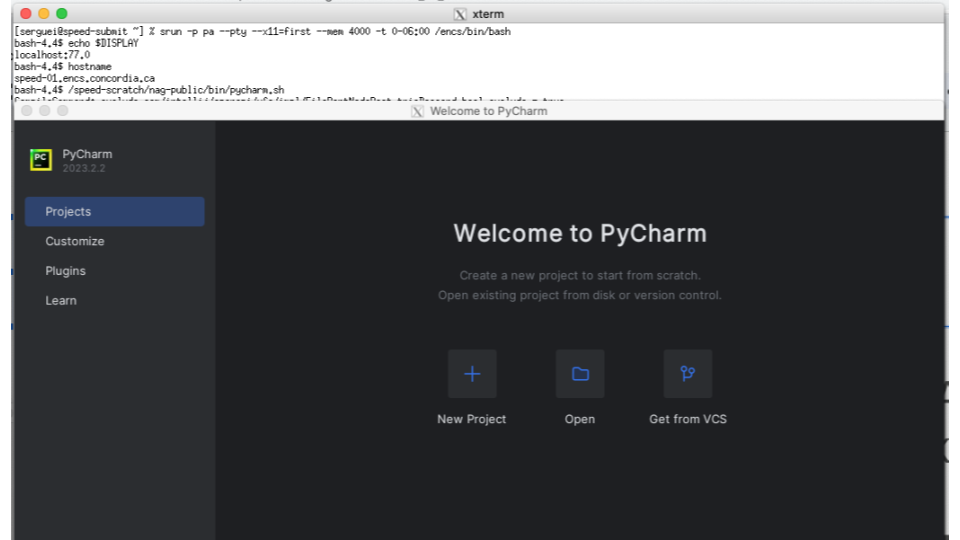
\includegraphics[width=\columnwidth]{images/pycharm}
		\caption{PyCharm Starting up on a Speed Node}
	\label{fig:pycharm}
\end{figure}

% ------------------------------------------------------------------------------
\subsubsection{Jupyter Notebooks}
\label{sect:jupyter}

This is an example of running Jupyter notebooks together with Singularity
(more on Singularity see \xs{sect:singularity-containers}).
Here we are using one of the OpenISS-derived containers (see \xs{sect:openiss-examples} as well).

\begin{enumerate}
\item
Use the \option{--x11} with \tool{salloc} or \tool{srun} as described in the above example

\item
Load Singularity module
\verb+module load singularity/3.10.4/default+

\item
Execute this Singularity command on a single line. It's best to save it in a shell script
that you could call, since it's long.
\scriptsize
\begin{verbatim}
srun singularity exec -B $PWD\:/speed-pwd,/speed-scratch/$USER\:/my-speed-scratch,/nettemp \
 --env SHELL=/bin/bash --nv /speed-scratch/nag-public/openiss-cuda-conda-jupyter.sif \
 /bin/bash -c '/opt/conda/bin/jupyter notebook --no-browser --notebook-dir=/speed-pwd \
 --ip="*" --port=8888 --allow-root'
\end{verbatim}
\normalsize

\item
Create an \tool{ssh} tunnel between your computer and the node (\texttt{speed-XX}) where Jupyter is
running (Using \texttt{speed-submit} as a ``jump server'') (Preferably: PuTTY, see \xf{fig:putty1} and \xf{fig:putty2})
\begin{verbatim}
ssh -L 8888:localhost:8888 speed-XX
\end{verbatim}
Don't close the tunnel.

\item
Open a browser, and copy your Jupyter's token, in the screenshot
example in \xf{fig:jupyter}; each time the token will be different,
as it printed to you in the terminal.

\small
\begin{verbatim}
http://localhost:8888/?token=5a52e6c0c7dfc111008a803e5303371ed0462d3d547ac3fb
\end{verbatim}
\normalsize

\item
Work with your notebook.

\end{enumerate}

\begin{figure}[htbp]
		\centering
		\fbox{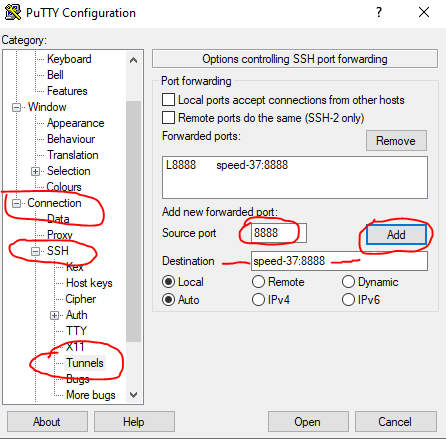
\includegraphics{images/putty1}}
	\caption{SSH tunnel configuration 1}
	\label{fig:putty1}
\end{figure}



\begin{figure}[htbp]
		\centering
		\fbox{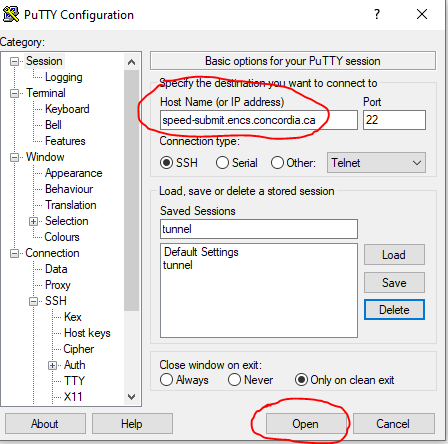
\includegraphics{images/putty2}}
	\caption{SSH tunnel configuration 2}
	\label{fig:putty2}
\end{figure}


\begin{figure}[htbp]
	\centering
	\fbox{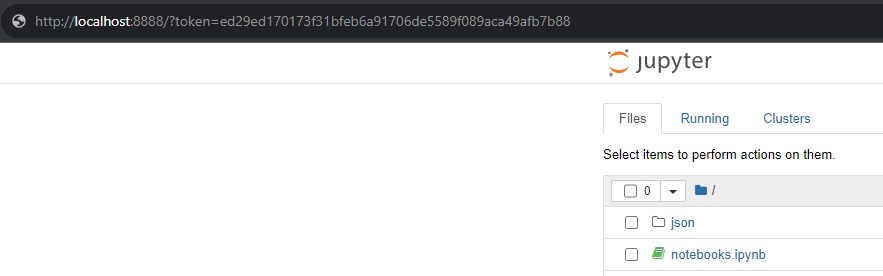
\includegraphics[width=1.00\textwidth]{images/jupyter.png}}
	\caption{Jupyter running on a Speed node}
	\label{fig:jupyter}
\end{figure}

% ------------------------------------------------------------------------------
\subsection{Scheduler Environment Variables}
\label{sect:env-vars}

The scheduler presents a number of environment variables that can be used in 
your jobs. You can invoke \tool{env} or \tool{printenv} in your
job to know what hose are (most begin with the prefix \texttt{SLURM}).
%
Some of the more useful ones are:
%\api{TMPDIR}, \api{SGE\_O\_WORKDIR}, and \api{NSLOTS}:

\begin{itemize}
\item
% TODO: verify temporal existence
\api{\$TMPDIR} -- the path to the job's temporary space on the node. It
\emph{only} exists for the duration of the job, so if data in the temporary space 
are important, they absolutely need to be accessed before the job terminates.

%\item
%\api{\$SGE\_O\_WORKDIR}=the path to the job's working directory (likely an
%NFS-mounted path). If, \texttt{-cwd}, was stipulated, that path is taken; if not, 
%the path defaults to your home directory.
\item
\api{\$SLURM\_SUBMIT\_DIR} -- the path to the job's working directory (likely an
NFS-mounted path). If, \option{--chdir}, was stipulated, that path is taken; if not, 
% TODO: verify if home or current:
the path defaults to your home directory.

% TODO: SLURM does not appear to have this
% SLURM_NTASKS
%\item
%\api{\$NSLOTS}=the number of cores requested for the job. This variable can 
%be used in place of hardcoded thread-request declarations. 

\item
\api{\$SLURM\_JOBID} -- your current jobs ID, useful for some manipulation
and reporting.

\item
\api{\$SLURM\_JOB\_NODELIST}=nodes participating in your job.

\item
\api{\$SLURM\_ARRAY\_TASK\_ID}=for array jobs (see \xs{sect:array-jobs}).

\item
See a more complete list here:

\small
\begin{itemize}
\item
\url{https://slurm.schedmd.com/srun.html#SECTION_INPUT-ENVIRONMENT-VARIABLES}
\item
\url{https://slurm.schedmd.com/srun.html#SECTION_OUTPUT-ENVIRONMENT-VARIABLES}
\end{itemize}
\normalsize

\end{itemize}

\noindent
In \xf{fig:tmpdir.sh} is a sample script, using some of these.

\begin{figure}[htpb]
    \lstinputlisting[language=csh,frame=single,basicstyle=\footnotesize\ttfamily]{tmpdir.sh}
    \caption{Source code for \file{tmpdir.sh}}
	\label{fig:tmpdir.sh}
\end{figure}

%

The final part of the job script involves the commands that will be executed by the job.
This section should include all necessary commands to set up and run the tasks
your script is designed to perform. You can use any Linux command in this section,
ranging from a simple executable call to a complex loop iterating through multiple commands.

\noindent \textbf{Best Practice}: prefix any compute-heavy step with \tool{srun}.
This ensures you gain proper insights on the execution of your job.

\noindent Each software program may have its own execution framework, as it's the script's author (e.g., you)
responsibility to review the software's documentation to understand its requirements.
Your script should be written to clearly specify the location of input and output files and the degree of parallelism needed.

\noindent Jobs that involve multiple interactions with data input and output files, should make use of \api{TMPDIR},
a scheduler-provided workspace nearly 1~TB in size.
\api{TMPDIR} is created on the local disk of the compute node at the start of a job, offering faster I/O operations
compared to shared storage (provided over NFS).

%TO BE DELETED 
% example in /home/n/nul-uge/templateTMPDIR.sh is not accessible.

%An sample job script using \api{TMPDIR} is available at \texttt{/home/n/nul-uge/templateTMPDIR.sh}: 
%the job is instructed to change to \api{\$TMPDIR}, to make the new directory \texttt{input}, to copy data from
%\texttt{\$SLURM\_SUBMIT\_DIR/references/} to \texttt{input/} (\api{\$SLURM\_SUBMIT\_DIR} represents the
%current working directory), to make the new directory \texttt{results}, to
%execute the program (which takes input from \texttt{\$TMPDIR/input/} and writes
%output to \texttt{\$TMPDIR/results/}), and finally to copy the total end results
%to an existing directory, \texttt{processed}, that is located in the current
%working directory.
% TODO: verify:
%\api{TMPDIR} only exists for the duration of the job, though,
%so it is very important to copy relevant results from it at job's end.

% includes:
%	2.2.1 Directives
%	2.2.2 Working with Modules
%	2.2.3 User Scripting

% 2.3 Sample Job Script
% -------------------------------------------------------------
% 2.3 Sample Job Script
% -------------------------------------------------------------
\subsection{Sample Job Script}
\label{sect:sample-job-script}

Here's a basic job script, \file{env.sh} shown in \xf{fig:env.sh}.
You can copy it from our \href{https://github.com/NAG-DevOps/speed-hpc}{GitHub repository}.

\small
\begin{figure}[htpb]
	\lstinputlisting[language=csh,frame=single,basicstyle=\ttfamily\scriptsize]{env.sh}
	\caption{Source code for \file{env.sh}}
	\label{fig:env.sh}
\end{figure}
\normalsize

\noindent The first line is the shell declaration (also know as a shebang) and sets the shell to \emph{tcsh}.
The lines that begin with \texttt{\#SBATCH} are directives for the scheduler.

\begin{itemize}
	\item \option{-J} (or \option{--job-name}) sets \emph{envs} as the job name.
	\item \option{--mail-type} sets the type of notifications.
	\item \option{--chdir} sets the working directory.
	\item \option{--nodes} specifies the number of required nodes.
	\item \option{--ntasks} specifies the number of tasks.
	\item \option{--cpus-per-task} requests 1 cpus.
	\item \option{--mem=} requests memory.

    \textbf{Note:} Jobs require the \option{--mem} option to be set either in the script
	or on the command line; \textbf{job submission will be rejected if it's missing.}
\end{itemize}

\noindent The script then:
\begin{enumerate}
    \item Creates a directory.
	\item Sets TMPDIR to a larger storage.
	\item Prints current date.
	\item Prints env variables.
	\item Prints current date again.
\end{enumerate}

\noindent The scheduler command, \tool{sbatch}, is used to submit (non-interactive) jobs.
From an ssh session on ``speed-submit'', submit this job with
\begin{verbatim}
    sbatch ./env.sh
\end{verbatim}

\noindent You will see, \texttt{Submitted batch job <JOB ID>}.
The commands \tool{squeue} and \tool{sinfo} can be used to look at the queue and the status of the cluster
%\texttt{squeue -l} and \texttt{sinfo -la}.

\small
\begin{verbatim}
[serguei@speed-submit src] % squeue -l
Thu Oct 19 11:38:54 2023
JOBID PARTITION     NAME     USER    STATE       TIME TIME_LIMI  NODES NODELIST(REASON)
 2641        ps interact   b_user   RUNNING   19:16:09 1-00:00:00      1 speed-07
 2652        ps interact   a_user   RUNNING      41:40 1-00:00:00      1 speed-07
 2654        ps envs       serguei  RUNNING       0:01 7-00:00:00      1 speed-07

[serguei@speed-submit src] % sinfo
PARTITION AVAIL  TIMELIMIT  NODES  STATE NODELIST
ps*          up 7-00:00:00      8  drng@ speed-[09-11,15-16,20-21,36]
ps*          up 7-00:00:00      3   drng speed-[38,42-43]
ps*          up 7-00:00:00      2  drain magic-node-[04,08]
ps*          up 7-00:00:00      4    mix magic-node-07,salus,speed-[07,37]
ps*          up 7-00:00:00      7  alloc magic-node-06,speed-[08,12,22-24,29]
ps*          up 7-00:00:00     13   idle magic-node-[05,09-10],speed-[19,30-35,39-41]
pg           up 7-00:00:00      1 drain* speed-05
pg           up 7-00:00:00      2    mix speed-[01,17]
pt           up 7-00:00:00      4   drng speed-[27,38,42-43]
pt           up 7-00:00:00      2    mix speed-[17,37]
pt           up 7-00:00:00      3   idle speed-[39-41]
pa           up 7-00:00:00      1   drng speed-27
pa           up 7-00:00:00      1    mix speed-01
pa           up 7-00:00:00      2   idle speed-[03,25]
cl           up 7-00:00:00      1 drain* speed-05
cl           up 7-00:00:00      4   drng speed-[27,38,42-43]
cl           up 7-00:00:00      3    mix speed-[01,17,37]
cl           up 7-00:00:00      6   idle speed-[03,19,25,39-41]
pc           up 7-00:00:00      1    mix salus
pm           up 7-00:00:00      2  drain magic-node-[04,08]
pm           up 7-00:00:00      1    mix magic-node-07
pm           up 7-00:00:00      1  alloc magic-node-06
pm           up 7-00:00:00      3   idle magic-node-[05,09-10]
pn           up 7-00:00:00      1  down* stellar
pn           up 7-00:00:00      2   idle matrix,nebulae
\end{verbatim}
\normalsize

Once the job finishes, there will be a new file in the directory that the job was started from,
with the syntax of, \texttt{slurm-<job id>.out}. This file represents the standard output
(and error, if there is any) of the job in question.
Important information is often written to this file.
%
%Congratulations on your first job!

% 2.4 Common Job Management Commands
% -------------------------------------------------------------
% 2.4 Common Job Management Commands
% -------------------------------------------------------------
\subsection{Common Job Management Commands}
\label{sect:job-management-commands}

Here is a summary of useful job management commands for handling various aspects of
job submission and monitoring on the Speed cluster:

\begin{itemize}
    \item Submitting a job:
	\begin{verbatim}
		sbatch -A <ACCOUNT> --mem=<MEMORY> -p <PARTITION> ./<myscript>.sh
	\end{verbatim}

	\item Checking your job(s) status:
	\begin{verbatim}
		squeue -u <ENCSusername>
	\end{verbatim}

	\item Displaying cluster status:
	\begin{verbatim}
		squeue
	\end{verbatim}
		\begin{itemize}
			\item Use \option{-A} for per account (e.g., \texttt{-A vidpro}, \texttt{-A aits})
			\item Use \option{-p} for per partition (e.g., \texttt{-p ps}, \texttt{-p pg}, \texttt{-p pt}), etc.
		\end{itemize}

	\item Displaying job information:
	\begin{verbatim}
		squeue --job <job-ID>
	\end{verbatim}

	\item Displaying individual job steps: (to see which step failed if you used \tool{srun})
	\begin{verbatim}
		squeue -las
	\end{verbatim}

	\item Monitoring job and cluster status: (view \tool{sinfo} and watch the queue for your job(s))
	\begin{verbatim}
		watch -n 1 "sinfo -Nel -pps,pt,pg,pa && squeue -la"
	\end{verbatim}

	\item Canceling a job:
	\begin{verbatim}
		scancel <job-ID>
	\end{verbatim}

	\item Holding a job:
	\begin{verbatim}
		scontrol hold <job-ID>
	\end{verbatim}

	\item Releasing a job:
	\begin{verbatim}
		scontrol release <job-ID>
	\end{verbatim}

	\item Getting job statistics: (including useful metrics like ``maxvmem'')
	\begin{verbatim}
		sacct -j <job-ID>
	\end{verbatim}
    \api{maxvmem} is one of the more useful stats that you can elect to display as a format option.

    \small
	\begin{verbatim}
	% sacct -j 2654
	JobID           JobName  Partition    Account  AllocCPUS      State ExitCode
	------------ ---------- ---------- ---------- ---------- ---------- --------
	2654               envs         ps     speed1          1  COMPLETED      0:0
	2654.batch        batch                speed1          1  COMPLETED      0:0
	2654.extern      extern                speed1          1  COMPLETED      0:0
	% sacct -j 2654 -o jobid,user,account,MaxVMSize,Reason%10,TRESUsageOutMax%30
	JobID             User    Account  MaxVMSize     Reason        TRESUsageOutMax
	------------ --------- ---------- ---------- ---------- ----------------------
	2654           serguei     speed1                  None
	2654.batch                 speed1    296840K             energy=0,fs/disk=1975
	2654.extern                speed1    296312K              energy=0,fs/disk=343
	\end{verbatim}
    \normalsize

	See \texttt{man sacct} or \texttt{sacct -e} for details of the available formatting options.
	You can define your preferred default format in the \api{SACCT\_FORMAT} environment variable
	in your \texttt{.cshrc} or \texttt{.bashrc} files.

	\item Displaying job efficiency: (including CPU and memory utilization)
	\begin{verbatim}
	    seff <job-ID>
	\end{verbatim}
    Don't execute it on \texttt{RUNNING} jobs (only on completed/finished jobs), else
	efficiency statistics may be misleading. If you define the following directive in your batch script,
    your GCS ENCS email address will receive an email with \tool{seff}'s output when your job is finished.
	\begin{verbatim}
	    #SBATCH --mail-type=ALL
	\end{verbatim}

	Output example:
	\begin{verbatim}
    Job ID: XXXXX
    Cluster: speed
    User/Group: user1/user1
    State: COMPLETED (exit code 0)
    Nodes: 1
    Cores per node: 4
    CPU Utilized: 00:04:29
    CPU Efficiency: 0.35% of 21:32:20 core-walltime
    Job Wall-clock time: 05:23:05
    Memory Utilized: 2.90 GB
    Memory Efficiency: 2.90% of 100.00 GB
	\end{verbatim}
\end{itemize}

% 2.5 Advanced sbatch Options
% -------------------------------------------------------------
% 2.5 Advanced sbatch Options
% -------------------------------------------------------------
\subsection{Advanced \tool{sbatch} Options}
\label{sect:submit-options}

In addition to the basic sbatch options presented earlier,
there are several advanced options that are generally useful:

\begin{itemize}
	\item E-mail notifications: requests the scheduler to send an email when the job changes state.
	\begin{verbatim}
		--mail-type=<TYPE>
	\end{verbatim}
	\texttt{<TYPE>} can be \texttt{ALL}, \texttt{BEGIN}, \texttt{END}, or \texttt{FAIL}.

	Mail is sent to the default address of \tool{<ENCSusername>@encs.concordia.ca}

	Which you can consult via \url{webmail.encs.concordia.ca} (use VPN from off-campus)
	unless a different address is supplied (see, \option{--mail-user}). The report sent when
    a job ends includes job runtime, as well as the maximum memory value hit (\api{maxvmem}).

    To specify a different email address for notifications rather than the default, use
    \begin{verbatim}
		--mail-user email@domain.com
	\end{verbatim}

	\item Export environment variables used by the script:
	\begin{verbatim}
		--export=ALL
		--export=NONE
		--export=VARIABLES
	\end{verbatim}

	\item Job runtime: sets a job runtime of min or HH:MM:SS. Note that if you give a single number,
	that represents \emph{minutes}, not hours. The set runtime should not exceed
	the default maximums of 24h for interactive jobs and 7 days for batch jobs.
	\begin{verbatim}
		-t <MINUTES> or DAYS-HH:MM:SS
	\end{verbatim}

	\item Job Dependencies: Runs the job only when the specified job \verb|<job-ID>| finishes.
    This is useful for creating job chains where subsequent jobs depend on the completion of previous ones.
	\begin{verbatim}
		--depend=<state:job-ID>
	\end{verbatim}
\end{itemize}

\noindent \textbf{Note:} \tool{sbatch} options can be specified during the job-submission command,
and these \emph{override} existing script options (if present). The syntax is
\begin{verbatim}
	sbatch [options] path/to/script
\end{verbatim}
but unlike in the script, the options are specified without the leading \verb+#SBATCH+
e.g.:
\begin{verbatim}
	sbatch -J sub-test --chdir=./ --mem=1G ./env.sh
\end{verbatim}

% 2.6 Array Jobs
% -------------------------------------------------------------
% 2.6 Array Jobs
% -------------------------------------------------------------
\subsection{Array Jobs}
\label{sect:array-jobs}

Array jobs are those that start a batch job or a parallel job multiple times.
Each iteration of the job array is called a task and receives a unique job ID.
Array jobs are particularly useful for running a large number of similar tasks with slight variations.

To submit an array job (Only supported for batch jobs),
use the \option{--array} option of the \tool{sbatch} command as follows:

\begin{verbatim}
	sbatch --array=n-m[:s] <script>
\end{verbatim}

\textbf{where}
\begin{itemize}
	\item \texttt{n}: indicates the start-id.
	\item \texttt{m}: indicates the max-id.
	\item \texttt{s}: indicates the step size.
\end{itemize}

\textbf{Examples:}
\begin{itemize}
	\item Submit a job with 1 task where the task-id is 10.
	\begin{verbatim}
		sbatch --array=10 array.sh
	\end{verbatim}

	\item Submit a job with 10 tasks numbered consecutively from 1 to 10.
	\begin{verbatim}
		sbatch --array=1-10 array.sh
	\end{verbatim}

	\item Submit a job with 5 tasks numbered consecutively with a step size of 3 (task-ids 3,6,9,12,15).
	\begin{verbatim}
		sbatch --array=3-15:3 array.sh
	\end{verbatim}

	\item Submit a job with 50000 elements, where \%a maps to the task-id between 1 and 50K.
	\begin{verbatim}
		sbatch --array=1-50000 -N1 -i my_in_%a -o my_out_%a array.sh
	\end{verbatim}
\end{itemize}

\textbf{Output files for Array Jobs:}
The default output and error-files are \texttt{slurm-job\_id\_task\_id.out}.
This means that Speed creates an output and an error-file for each task generated by the array-job,
as well as one for the super-ordinate array-job.
To alter this behavior use the \option{-o} and \option{-e} options of \tool{sbatch}.

For more details about Array Job options, please review the manual pages for \tool{sbatch}
by executing the following at the command line on \tool{speed-submit}.
\begin{verbatim}
    man sbatch
\end{verbatim}

% 2.7 Requesting Multiple Cores (i.e., Multithreading Jobs)
% -------------------------------------------------------------
% 2.7 Requesting Multiple Cores (i.e., Multithreading Jobs)
% -------------------------------------------------------------
\subsection{Requesting Multiple Cores (i.e., Multithreading Jobs)}
\label{sect:multicore-jobs}

For jobs that can take advantage of multiple machine cores, you can
request up to 32 cores (per job) in your script using the following options:

\begin{verbatim}
	#SBATCH -n      #cores for processes>
	#SBATCH -n 1
	#SBATCH -c      #cores for threads of a single process
\end{verbatim}

\noindent Both \tool{sbatch} and \tool{salloc} support \option{-n} on the command line,
and it should always be used either in the script or on the command line as the
default $n=1$.

\textbf{Important Considerations}:
\begin{itemize}
	\item Do not request more cores than you think will be useful,
	as larger-core jobs are more difficult to schedule.

	\item If you are running a program that scales out to the maximum single-machine core count available,
    please request 32 cores to avoid node oversubscription (i.e., overloading the CPUs).
\end{itemize}

\textbf{Note:}
\begin{itemize}
    \item\option{--ntasks} or \option{--ntasks-per-node}
    (\option{-n}) refers to processes (usually the ones run with \tool{srun}).
    \item \option{--cpus-per-task} (\option{-c}) corresponds to threads per process.
\end{itemize}

\noindent Some programs consider them equivalent, while others do not.
For example, Fluent uses \option{--ntasks-per-node=8} and \option{--cpus-per-task=1},
whereas others may set \option{--cpus-per-task=8} and \option{--ntasks-per-node=1}.
If one of these is not 1, some applications need to be configured to use \texttt{n * c} total cores.

\noindent Core count associated with a job appears under,``AllocCPUS'', in the, \texttt{sacct -j <job-id>}, output.

\small
\begin{verbatim}
	[serguei@speed-submit src] % squeue -l
	Thu Oct 19 20:32:32 2023
	JOBID PARTITION     NAME     USER    STATE       TIME TIME_LIMI  NODES NODELIST(REASON)
	2652        ps interact   a_user  RUNNING   9:35:18 1-00:00:00      1 speed-07
	[serguei@speed-submit src] % sacct -j 2652
	JobID           JobName  Partition    Account  AllocCPUS      State ExitCode
	------------ ---------- ---------- ---------- ---------- ---------- --------
	2652         interacti+         ps     speed1         20    RUNNING      0:0
	2652.intera+ interacti+                speed1         20    RUNNING      0:0
	2652.extern      extern                speed1         20    RUNNING      0:0
	2652.0       gydra_pmi+                speed1         20  COMPLETED      0:0
	2652.1       gydra_pmi+                speed1         20  COMPLETED      0:0
	2652.2       gydra_pmi+                speed1         20     FAILED      7:0
	2652.3       gydra_pmi+                speed1         20     FAILED      7:0
	2652.4       gydra_pmi+                speed1         20  COMPLETED      0:0
	2652.5       gydra_pmi+                speed1         20  COMPLETED      0:0
	2652.6       gydra_pmi+                speed1         20  COMPLETED      0:0
	2652.7       gydra_pmi+                speed1         20  COMPLETED      0:0
\end{verbatim}
\normalsize

% 2.8 Interactive Jobs
% -------------------------------------------------------------
% 2.8 Interactive Jobs
% -------------------------------------------------------------
\subsection{Interactive Jobs}
\label{sect:interactive-jobs}

Interactive job sessions allow you to interact with the system in real-time.
These sessions are particularly useful for tasks such as testing, debugging, optimizing code,
setting up environments, and other preparatory work before submitting batch jobs.

%  2.8.1 Command Line
% -------------------
\subsubsection{Command Line}
\label{sect:command-line}

To request an interactive job session, use the \texttt{salloc} command with appropriate options.
This is similar to submitting a batch job but allows you to run shell commands interactively
within the allocated resources. For example:
\begin{verbatim}
	salloc -J interactive-test --mem=1G -p ps -n 8
\end{verbatim}

Within the allocated \tool{salloc} session, you can run shell commands as usual.
It is recommended to use \tool{srun} for compute-intensive steps within \tool{salloc}.
If you need a quick, short job just to compile something on a GPU node,
you can use an interactive srun directly. For example, a 1-hour allocation:

\textbf{For tcsh}:
\begin{verbatim}
	srun --pty -n 8 -p pg --gpus=1 --mem=1G -t 60 /encs/bin/tcsh
\end{verbatim}
\textbf{For bash}:
\begin{verbatim}
	srun --pty -n 8 -p pg --gpus=1 --mem=1G -t 60 /encs/bin/bash
\end{verbatim}

% 2.8.2 Graphical Applications
% -----------------------------
\subsubsection{Graphical Applications}
\label{sect:graphical-applications}

To run graphical UI applications (e.g., MALTLAB, Abaqus CME, IDEs like PyCharm, VSCode, Eclipse, etc.) on Speed,
you need to enable X11 forwarding from your client machine Speed then to the compute node.
To do so, follow these steps:
\begin{enumerate}
\item Run an X server on your client machine:
\begin{itemize}
    \item \textbf{Windows:} Use MobaXterm with X turned on, or Xming + PuTTY with X11 forwarding, or XOrg under Cygwin
    \item \textbf{macOS:} Use XQuarz -- use its \tool{xterm} and \texttt{ssh -X}
    \item \textbf{Linux:} Use \texttt{ssh -X speed.encs.concordia.ca}
\end{itemize}
For more details, see \href{https://www.concordia.ca/ginacody/aits/support/faq/xserver.html}{How do I remotely launch X(Graphical) applications?}

\item Verify that X11 forwarding is enabled by printing the \api{DISPLAY} variable:
\begin{verbatim}
    echo $DISPLAY
\end{verbatim}

\item Start an interactive session with X11 forwarding enabled (Use the \option{--x11} with \tool{salloc} or \tool{srun}), for example:
\begin{verbatim}
    salloc -p ps --x11=first --mem=4G -t 0-06:00
\end{verbatim}

\item Once landed on a compute node, verify \api{DISPLAY} again.

\item Set the \api{XDG\_RUNTIME\_DIR} variable to a directory in your \tool{speed-scratch} space:
\begin{verbatim}
    mkdir -p /speed-scratch/$USER/run-dir
    setenv XDG_RUNTIME_DIR /speed-scratch/$USER/run-dir
\end{verbatim}

\item Launch your graphical application:
\begin{verbatim}
    module load matlab/R2023a/default
    matlab
\end{verbatim}
\end{enumerate}

\noindent\textbf{Note:} with X11 forwarding the graphical rendering is happening on your client machine!
That is you are not using GPUs on Speed to render graphics,
instead all graphical information is forwarded from Speed to your desktop or laptop over X11,
which in turn renders it using its own graphics card. Thus, for GPU rendering jobs either keep them
non-interactive or use VirtualGL.

\noindent Here's an example of starting PyCharm (see \xf{fig:pycharm}).
\textbf{Note:} If using VSCode, it's currently only supported with the \tool{--no-sandbox} option.

\textbf{TCSH version:}
\small
\begin{verbatim}
    ssh -X speed (XQuartz xterm, PuTTY or MobaXterm have X11 forwarding too)
    [speed-submit] [/home/c/carlos] > echo $DISPLAY
    localhost:14.0
    [speed-submit] [/home/c/carlos] > cd /speed-scratch/$USER
    [speed-submit] [/speed-scratch/carlos] > echo $DISPLAY
    localhost:13.0
    [speed-submit] [/speed-scratch/carlos] > salloc -pps --x11=first --mem=4Gb -t 0-06:00
    [speed-07] [/speed-scratch/carlos] > echo $DISPLAY
    localhost:42.0
    [speed-07] [/speed-scratch/carlos] > hostname
    speed-07.encs.concordia.ca
    [speed-07] [/speed-scratch/carlos] > setenv XDG_RUNTIME_DIR /speed-scratch/$USER/run-dir
    [speed-07] [/speed-scratch/carlos] > /speed-scratch/nag-public/bin/pycharm.sh
\end{verbatim}
\normalsize

\textbf{BASH version:}
\small
    \begin{verbatim}
    bash-3.2$ ssh -X speed (XQuartz xterm, PuTTY or MobaXterm have X11 forwarding too)
    serguei@speed's password:
    [serguei@speed-submit ~] % echo $DISPLAY
    localhost:14.0
    [serguei@speed-submit ~] % salloc -p ps --x11=first --mem=4Gb -t 0-06:00
    bash-4.4$ echo $DISPLAY
    localhost:77.0
    bash-4.4$ hostname
    speed-01.encs.concordia.ca
    bash-4.4$ export XDG_RUNTIME_DIR=/speed-scratch/$USER/run-dir
    bash-4.4$ /speed-scratch/nag-public/bin/pycharm.sh
\end{verbatim}
\normalsize

\begin{figure}[htpb]
	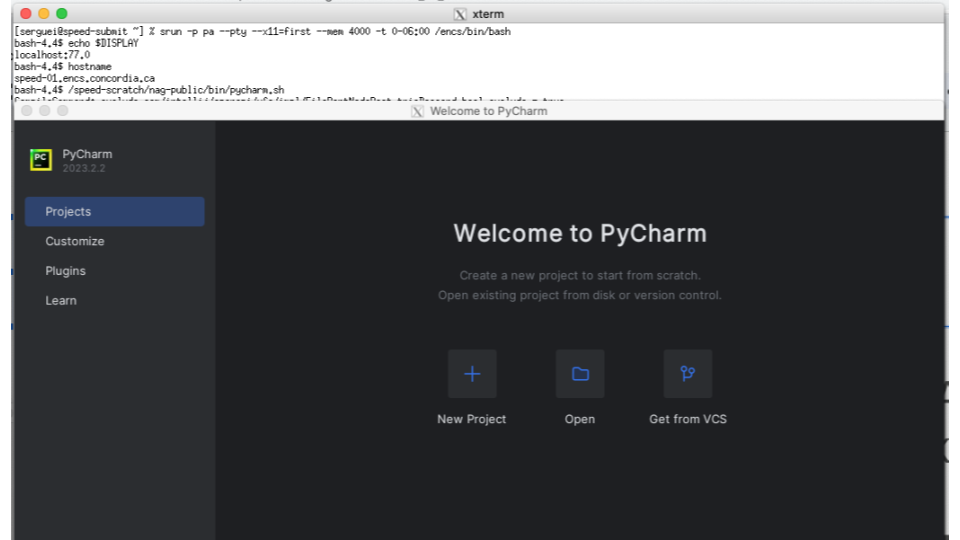
\includegraphics[width=\columnwidth]{images/pycharm}
	\caption{Launching PyCharm on a Speed Node}
	\label{fig:pycharm}
\end{figure}

% 2.8.3 Jupyter Notebooks
% ------------------------
\subsubsection{Jupyter Notebooks}
\label{sect:jupyter-notebooks}

% 2.8.3.1 Jupyter Notebook in Singularity
% ---------------------------------------
\paragraph{Jupyter Notebook in Singularity}
\label{sect:jupyter-singularity}
\noindent To run Jupyter Notebooks using Singularity (more on Singularity see \xs{sect:singularity-containers}),
follow these steps:

\begin{enumerate}
% X11 is not really needed for Jupyter since we tunnel and use a browser
%\item Connect to Speed with X11 forwarding enabled:
\item Connect to Speed, e.g. interactively, using \tool{salloc}
%\item Use the \option{--x11} with \tool{salloc} or \tool{srun} as described in the above example
\item Load Singularity module
    \verb+module load singularity/3.10.4/default+

\item Execute this Singularity command on a single line or save it in a shell script from our
\href{https://github.com/NAG-DevOps/speed-hpc/blob/master/src/jupyter.sh}{GitHub repo}
where you could easily invoke it.

\small
\begin{verbatim}
srun singularity exec -B $PWD\:/speed-pwd,/speed-scratch/$USER\:/my-speed-scratch,/nettemp \
--env SHELL=/bin/bash --nv /speed-scratch/nag-public/openiss-cuda-conda-jupyter.sif \
/bin/bash -c '/opt/conda/bin/jupyter notebook --no-browser --notebook-dir=/speed-pwd \
--ip="*" --port=8888 --allow-root'
\end{verbatim}
\normalsize

\item In a new terminal window, create an \tool{ssh} tunnel between your computer and the node (\texttt{speed-XX}) where Jupyter is
running (using \texttt{speed-submit} as a ``jump server'', see, e.g., in PuTTY, in \xf{fig:putty1} and \xf{fig:putty2})
\small
\begin{verbatim}
    ssh -L 8888:speed-XX:8888 <ENCS-username>@speed-submit.encs.concordia.ca
\end{verbatim}
\normalsize
\textbf{Don't close the tunnel after establishing.}

\item Open a browser, and copy your Jupyter's token (it's printed to you in the terminal)
and paste it in the browser's URL field. In our case, the URL is:
\small
\begin{verbatim}
    http://localhost:8888/?token=5a52e6c0c7dfc111008a803e5303371ed0462d3d547ac3fb
\end{verbatim}
\normalsize

\item Access the Jupyter Notebook interface in your browser.
\end{enumerate}

\begin{figure}[htbp]
	\centering
	\fbox{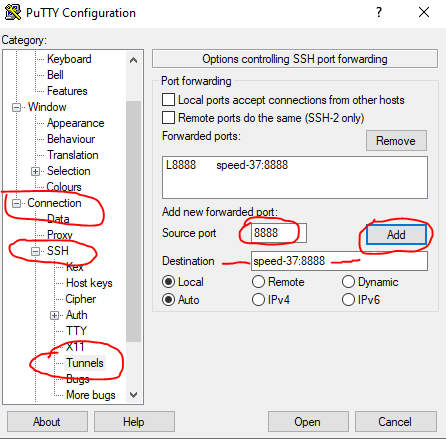
\includegraphics{images/putty1}}
	\caption{SSH tunnel configuration 1}
	\label{fig:putty1}
\end{figure}

\begin{figure}[htbp]
	\centering
	\fbox{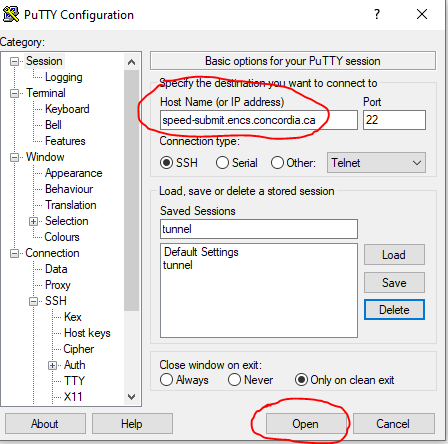
\includegraphics{images/putty2}}
	\caption{SSH tunnel configuration 2}
	\label{fig:putty2}
\end{figure}

\begin{figure}[htbp]
	\centering
	\fbox{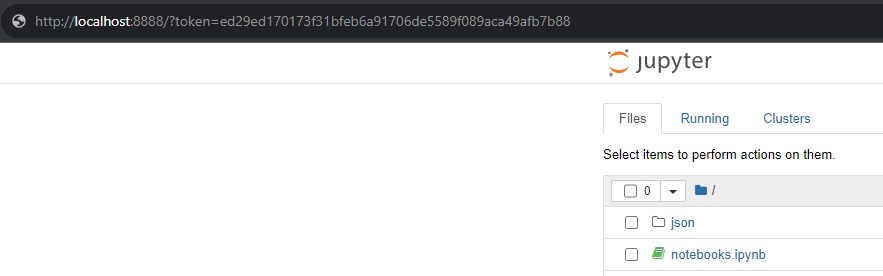
\includegraphics[width=0.9\textwidth]{images/jupyter.png}}
	\caption{Jupyter running on a Speed node}
	\label{fig:jupyter}
\end{figure}

\noindent Another sample is the OpenISS-derived containers with Conda and Jupyter,
see \xs{sect:openiss-examples} for details.

% 2.8.3.2 Jupyter Notebook in Conda
% ----------------------------------
\paragraph{Jupyter Notebook in Conda}
\label{sect:jupyter-conda}

For setting up Jupyter Labs with Conda and Pytorch, follow these steps:

\textbf{Environment preparation:} (only once, takes some time to run to install all required dependencies)
\begin{enumerate}
\item Start an interactive session, and navigate to your \tool{speed-scratch} directory:
\begin{verbatim}
salloc --mem=20G --gpus=1
cd /speed-scratch/$USER
\end{verbatim}

\item Load and initilize the environment
\begin{verbatim}
module load anaconda/2023.03/default
conda init tcsh
source ~/.tcshrc
\end{verbatim}

\item Set up Conda environment by runnung \tool{setup-conda.sh}
(on the compute node salloc brought you to, not on speed-submit)
as shown in \xf{fig:setup_conda.sh}
\begin{verbatim} ./setup_conda.sh \end{verbatim}

\small
\begin{figure}[htpb]
    \lstinputlisting[language=csh,frame=single,basicstyle=\ttfamily\scriptsize]{../../src/jupyterlabs/setup_conda.sh}
    \caption{Source code for \file{setup_conda.sh}}
    \label{fig:setup_conda.sh}
\end{figure}
\normalsize
\end{enumerate}

The script will:
\begin{itemize}
    \item create a Jupyter directory change Jupyter to any name of your choice in the script
    \item set environment variables
    \item create a conda environment named jupyter-env
    \item install JupyterLabs and pytorch
    \item exit the interactive session
\end{itemize}

\textbf{Launching Jupyter Labs instance from \textbf{speed-submit}:}
\begin{enumerate}
    \item Run the \tool{start\_jupyterlab.sh} script each time you need to launch JupyterLab from the submit node
    The script will:
    \begin{itemize}
        \item allocate resources for your job on a compute node
        \item start jupyter server by running \tool{run\_jupyterlab.sh}
        \item print the ssh command that you can use to connect to the compute node runnung the jupyter notebook (this is done in a new terminal)
        \item print the token/link to the jupyter server to paste in a web browser (starting with http://127.0.0.1/...)
    \end{itemize}

    \item Open a browser, and copy your Jupyter's token and paste it in the browser's URL field.
\end{enumerate}


% 2.8.3.3 Jupyter Notebook in Python Virtual Env
% ----------------------------------------------
\paragraph{Jupyter Notebook in Python venv}
\label{sect:jupyter-python}

This is an example of Jupyter Labs running in a Python Virtual environment on Speed.

\textbf{Note:} Use of Python virtual environments is preferred over Conda at Alliance Canada clusters.
If you prefer to make jobs that are more compatible between Speed and Alliance clusters, use Python
\texttt{venv}s. See \url{https://docs.alliancecan.ca/wiki/Anaconda/en}
and \url{https://docs.alliancecan.ca/wiki/JupyterNotebook}.

\begin{itemize}
\item Environment preparation: for the FIRST time only:
\begin{enumerate}
\item Go to your speed-scratch directory: \texttt{cd /speed-scratch/\$USER}
\item Open an interactive session: \texttt{salloc --mem=50G --gpus=1 --constraint=el9}
\item Create a Python \texttt{venv} and install \tool{jupyterlab}+\tool{pytorch}
\small
\begin{verbatim}
module load python/3.11.5/default
setenv TMPDIR /speed-scratch/$USER/tmp
setenv TMP /speed-scratch/$USER/tmp
setenv PIP_CACHE_DIR /speed-scratch/$USER/tmp/cache
python -m venv /speed-scratch/$USER/tmp/jupyter-venv
source /speed-scratch/$USER/tmp/jupyter-venv/bin/activate.csh
pip install jupyterlab
pip3 install torch torchvision torchaudio --index-url https://download.pytorch.org/whl/cu118
exit
\end{verbatim}
\normalsize
\end{enumerate}

\item Running Jupyter, from \textbf{speed-submit}:
\begin{enumerate}
\item Open an interactive session: \texttt{salloc --mem=50G --gpus=1 --constraint=el9}
\small
\begin{verbatim}
cd /speed-scratch/$USER
module load python/3.11.5/default
setenv PIP_CACHE_DIR /speed-scratch/$USER/tmp/cache
source /speed-scratch/$USER/tmp/jupyter-venv/bin/activate.csh
jupyter lab --no-browser --notebook-dir=$PWD --ip="0.0.0.0" --port=8888 --port-retries=50
\end{verbatim}
\normalsize

\item Verify which port the system has assigned to Jupyter: \texttt{http://localhost:XXXX/lab?token=}

\item SSH Tunnel creation: similar to Jupyter in Singularity, see \xs{sect:jupyter-singularity}

\item Open a browser and type: \texttt {localhost:XXXX} (using the port assigned)
\end{enumerate}
\end{itemize}


% 2.8.4 Visual Studio Code
% ------------------------
\subsubsection{Visual Studio Code}
\label{sect:vscode}

This is an example of running VScode, it's similar to Jupyter notebooks, but
it doesn't use containers. \textbf{Note:} this a Web-based version; there exists the local
(workstation)~--~remote (speed-node) client-server version too, but it is for advanced users
and is out of scope here (so no support, use it at your own risk).

\begin{itemize}
\item Environment preparation: for the FIRST time:
\begin{enumerate}
    \item Go to your speed-scratch directory: \texttt{cd /speed-scratch/\$USER}
    \item Create a vscode directory: \texttt{mkdir vscode}
    \item Create another directory: \texttt{mkdir -p /speed-scratch/\$USER/run-user}
\end{enumerate}

\item Running VScode
\begin{enumerate}
    \item Go to your vscode directory:
    \texttt{cd /speed-scratch/\$USER/vscode}
    \item Open interactive session:
    \texttt{salloc --mem=10Gb --constraint=el9}
    \item Set environment variable:
    \texttt{setenv XDG\_RUNTIME\_DIR /speed-scratch/\$USER/run-user}
    \item Run VScode, change the port if needed.
    \scriptsize
    \begin{verbatim}
/speed-scratch/nag-public/code-server-4.22.1/bin/code-server --user-data-dir=$PWD\/projects \
--config=$PWD\/home/.config/code-server/config.yaml --bind-addr="0.0.0.0:8080" $PWD\/projects
    \end{verbatim}
    \normalsize
    \item SSH Tunnel creation: similar to Jupyter, see \xs{sect:jupyter-singularity}
    \item Open a browser and type: \texttt{localhost:8080}
    \item If the browser asks for a password, consult:
    \begin{verbatim}
    cat /speed-scratch/$USER/vscode/home/.config/code-server/config.yaml
    \end{verbatim}
\end{enumerate}
\end{itemize}

\begin{figure}[htbp]
	\centering
	\fbox{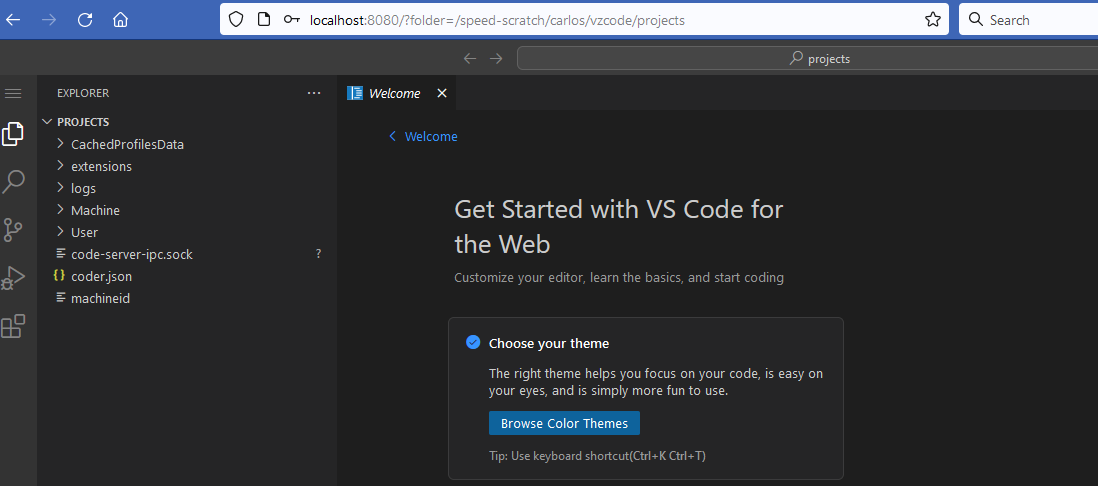
\includegraphics[width=0.9\textwidth]{images/vscode.png}}
	\caption{VScode running on a Speed node}
	\label{fig:vscode}
\end{figure}

% includes:
%	2.8.1 Command Line
%	2.8.2 Graphical Applications
%	2.8.3 Jupyter Notebooks
%		2.8.3.1 Jupyter Notebook in Singularity
%		2.8.3.2 Jupyter Notebook in Conda
%		2.8.3.3 Jupyter Notebook in Python Virtual Env
%	2.8.4 Visual Studio Code

% 2.9 Scheduler Environment Variables
% -------------------------------------------------------------
% 2.9 Scheduler Environment Variables
% -------------------------------------------------------------
\subsection{Scheduler Environment Variables}
\label{sect:env-vars}

The scheduler provides several environment variables that can be useful in your job scripts.
These variables can be accessed within the job using commands like \tool{env} or \tool{printenv}.
Many of these variables start with the prefix \texttt{SLURM}.

\noindent Here are some of the most useful environment variables:

\begin{itemize}
	\item
	\api{\$TMPDIR} (and \api{\$SLURM\_TMPDIR}):
	% TODO: verify temporal existence
	This is the path to the job's temporary space on the node. It \emph{only} exists for the duration of the job.
	If you need the data from this temporary space, ensure you copy it before the job terminates.

	\item
	\api{\$SLURM\_SUBMIT\_DIR}:
	The path to the job's working directory (likely an NFS-mounted path).
	If, \option{--chdir}, was stipulated, that path is taken; if not,
	the path defaults to your home directory.

	\item
	\api{\$SLURM\_JOBID}:
	This variable holds the current job's ID, which is useful for job
	manipulation and reporting within the job's process.

	\item
	\api{\$SLURM\_NTASKS}: the number of cores requested for the job. This variable can
	be used in place of hardcoded thread-request declarations, e.g., for
	Fluent or similar.

	\item
	\api{\$SLURM\_JOB\_NODELIST}:
	This lists the nodes participating in your job.

	\item \api{\$SLURM\_ARRAY\_TASK\_ID}:
	For array jobs, this variable represents the task ID
	(refer to \xs{sect:array-jobs} for more details on array jobs).
\end{itemize}

\noindent For a more comprehensive list of environment variables,
refer to the SLURM documentation for
\href{https://slurm.schedmd.com/srun.html#SECTION_INPUT-ENVIRONMENT-VARIABLES}{Input Environment Variables} and
\href{https://slurm.schedmd.com/srun.html#SECTION_OUTPUT-ENVIRONMENT-VARIABLES}{Output Environment Variables}.

\noindent An example script that utilizes some of these environment variables
is in \xf{fig:tmpdir.sh}.

\begin{figure}[htpb]
    \lstinputlisting[language=csh,frame=single,basicstyle=\scriptsize\ttfamily]{tmpdir.sh}
    \caption{Source code for \file{tmpdir.sh}}
	\label{fig:tmpdir.sh}
\end{figure}

% 2.10 SSH Keys for MPI
% -------------------------------------------------------------
% 2.10 SSH Keys for MPI
% -------------------------------------------------------------
\subsection{SSH Keys for MPI}
\label{sect:ssh-mpi}

Some programs, such as Fluent, utilize MPI (Message Passing Interface) for parallel processing.
MPI requires `passwordless login', which is achieved through SSH keys.
Here are the steps to set up SSH keys for MPI:

\begin{itemize}
	\item Navigate to the \texttt{.ssh} directory
	\begin{verbatim}
	cd ~/.ssh
	\end{verbatim}

	\item Generate a new SSH key pair (Accept the default location and leave the passphrase blank)
	\begin{verbatim}
	ssh-keygen -t ed25519
	\end{verbatim}

	\item Authorize the Public Key:
	\begin{verbatim}
	cat id_ed25519.pub >> authorized_keys
	\end{verbatim}
	If the \texttt{\href{https://www.ssh.com/academy/ssh/authorized-keys-file}{authorized\_keys}} file does not exist, use
	\begin{verbatim}
	cat id_ed25519.pub > authorized_keys
	\end{verbatim}

	\item Set permissions: ensure the correct permissions are set for the `authorized\_keys' file and your home directory
	(most users will already have these permissions by default):
	\begin{verbatim}
	chmod 600 ~/.ssh/authorized_keys
	chmod 700 ~
	\end{verbatim}
\end{itemize}

% 2.11 Creating Virtual Environments
% -------------------------------------------------------------
% 2.11 Creating Virtual Environments
% -------------------------------------------------------------
\subsection{Creating Virtual Environments}
\label{sect:creating-venvs}
\label{sect:environments}
\label{sect:examples-venv}

The following documentation is specific to \textbf{Speed}, other clusters may have their own requirements.
%HPC Facility at the Gina Cody School of Engineering and Computer Science.

Virtual environments are typically created using Conda or Python.
Another option is Singularity (detailed in \xs{sect:singularity-containers}).
These environments are usually created once during an interactive session before
submitting a batch job to the scheduler.

The job script submitted to the scheduler should:
\begin{enumerate}
	\item Activate the virtual environment.
	\item Use the virtual environment.
	\item Deactivate the virtual environment at the end of the job.
\end{enumerate}

%  2.11.1 Anaconda
% -------------------
\subsubsection{Anaconda}
\label{sect:conda-venv}

To create an Anaconda environment, follow these steps:
\begin{enumerate}
	\item Request an interactive session
	\begin{verbatim}
		salloc -p pg --gpus=1
	\end{verbatim}

	\item Load the Anaconda module and create your Anaconda environment in your speed-scratch directory by using
	the \option{--prefix} option (without this o tion, the environment will be created in your home directory by default).
	\begin{verbatim}
		module load anaconda3/2023.03/default
		conda create --prefix /speed-scratch/$USER/myconda
	\end{verbatim}

	\item List environments (to view your conda environment)
	\begin{verbatim}
		conda info --envs
		# conda environments:
		#
		base                  *  /encs/pkg/anaconda3-2023.03/root
                         		 /speed-scratch/a_user/myconda
	\end{verbatim}

	\item Activate the environment
	\begin{verbatim}
		conda activate /speed-scratch/$USER/myconda
	\end{verbatim}

	\item Add \tool{pip} to your environment (this will install \tool{pip} and \tool{pip}'s dependencies,
	including \tool{python}, into the environment.)
	\begin{verbatim}
		conda install pip
	\end{verbatim}
\end{enumerate}

\noindent A consolidated example using Conda:
\begin{verbatim}
    salloc --mem=10G --gpus=1 -p pg -A <slurm account name>
    mkdir -p /speed-scratch/$USER
    cd /speed-scratch/$USER
    module load anaconda3/2023.03/default
    conda create -p /speed-scratch/$USER/pytorch-env
    conda activate /speed-scratch/$USER/pytorch-env
    conda install python=3.11.0
    pip3 install torch torchvision torchaudio --index-url \
    https://download.pytorch.org/whl/cu117
    ....
    conda deactivate
    exit # end the salloc session
\end{verbatim}

\noindent If you encounter \textbf{no space left error} while creating Conda environments, please refer to
\xa{sect:quota-exceeded}.
Likely you forgot \option{--prefix} or environment variables below.

\textbf{Important Note:} \tool{pip} (and \tool{pip3}) are package installers for Python. When you use
\texttt{pip install}, it installs packages from the Python Package Index (PyPI), whereas,
\texttt{conda install} installs packages from Anaconda's repository.

\paragraph{Conda Env without \option{--prefix}}

If you don't want to use the \option{--prefix} option every time you create a new environment and
do not want to use the default home directory, you can create a new directory and set the following
variables to point to the newly created directory, e.g.:
\begin{verbatim}
    mkdir -p /speed-scratch/$USER/conda
    setenv CONDA_ENVS_PATH /speed-scratch/$USER/conda
    setenv CONDA_PKGS_DIRS /speed-scratch/$USER/conda/pkg
\end{verbatim}

\noindent If you want to make these changes permanent, add the variables to your \texttt{.tcshrc}
or \texttt{.bashrc} (depending on the default shell you are using).


% 2.11.2 Python
% -------------------
\subsubsection{Python}
\label{sect:python-venv}

Setting up a Python virtual environment is straightforward.
Here's an example that use a Python virtual environment:

\begin{verbatim}
    salloc --mem=10G --gpus=1 -p pg -A <slurm account name>
    mkdir -p /speed-scratch/$USER
    cd /speed-scratch/$USER
    module load python/3.9.1/default
    mkdir -p /speed-scratch/$USER/tmp
    setenv TMPDIR /speed-scratch/$USER/tmp
    setenv TMP /speed-scratch/$USER/tmp
    python -m venv $TMPDIR/testenv (testenv=name of the virtualEnv)
    source /speed-scratch/$USER/tmp/testenv/bin/activate.csh
    pip install <modules>
    deactivate
    exit
\end{verbatim}

\noindent See, e.g.,
\href{https://github.com/NAG-DevOps/speed-hpc/blob/master/src/gurobi-with-python.sh}
{\texttt{gurobi-with-python.sh}}

\noindent\textbf{Important Note:} our partition \texttt{ps} is used for CPU jobs, while \texttt{pg},
\texttt{pt}, and \texttt{cl} are used for GPU jobs. You do not need to use \option{--gpus}
when preparing environments for CPU jobs.

\noindent\textbf{Note:} Python enviornments are also preferred over Conda
in some clusters, see a note in~\xs{sect:jupyter-python}.

% includes:
%	2.11.1 Anaconda
%		2.11.1.1 Conda Env without --prefix
%	2.11.2 Python

% 2.12 Example Job Script: Fluent
% -------------------------------------------------------------
% 2.12 Example Job Script: Fluent
% -------------------------------------------------------------
% TODO: delete the file
%% -------------- 2.12 Example Job Script: Fluent --------------
% -------------------------------------------------------------
\subsection{Example Job Script: Fluent}

\begin{figure}[htpb]
  \lstinputlisting[language=csh,frame=single,basicstyle=\footnotesize\ttfamily]{fluent.sh}
  \caption{Source code for \texttt{fluent.sh}}
  \label{fig:fluent.sh}
\end{figure}

The job script in \xf{fig:fluent.sh} runs Fluent in parallel over 32 cores. 
Notable aspects of this script include requesting e-mail notifications (\option{--mail-type}), 
defining the parallel environment for Fluent with \option{-t\$SLURM\_NTASKS} and \option{-g-cnf=\$FLUENTNODES}, 
and setting \api{\$TMPDIR} as the in-job location for the ``moment'' \file{rfile.out} file.
The script also copies everything from \api{\$TMPDIR} to a directory in the user's NFS-mounted home after the job completes.
Job progress can be monitored by examining the standard-out file (e.g.,
\texttt{slurm-249.out}), and/or by examining the ``moment'' file in TMPDIR (usually
\texttt{/disk/nobackup/<yourjob>} (it starts with your job-ID)) on the node running
the job. Be cautious with journal-file paths.

% -------------- 2.13 Example Job Script: EfficientDet --------
% -------------------------------------------------------------
\subsection{Example Job: EfficientDet}

The following steps describe how to create an EfficientDet environment on Speed, 
as submitted by a member of Dr. Amer's research group:

\begin{itemize}
  \item Navigate to your \texttt{speed-scratch} directory:
  \begin{verbatim}
	cd /speed-scratch/$USER
  \end{verbatim}
  \item Load Python module
  \begin{verbatim}
	module load python/3.8.3
  \end{verbatim}
  \item Create and activate the virtual environment
  \begin{verbatim}
	python3 -m venv <env_name>
	source <env_name>/bin/activate.csh
  \end{verbatim}
  \item Install DL packages for EfficientDet
  \small
  \begin{verbatim}
	pip install tensorflow==2.7.0
	pip install lxml>=4.6.1
	pip install absl-py>=0.10.0
	pip install matplotlib>=3.0.3
	pip install numpy>=1.19.4
	pip install Pillow>=6.0.0
	pip install PyYAML>=5.1
	pip install six>=1.15.0
	pip install tensorflow-addons>=0.12
	pip install tensorflow-hub>=0.11
	pip install neural-structured-learning>=1.3.1
	pip install tensorflow-model-optimization>=0.5
	pip install Cython>=0.29.13
	pip install git+https://github.com/cocodataset/cocoapi.git#subdirectory=PythonAPI
	\end{verbatim}
  \normalsize
\end{itemize}

% -------------- 2.14 Java Jobs -------------------------------
% -------------------------------------------------------------
\subsection{Java Jobs}
\label{sect:java}

Jobs that call Java have a memory overhead, which needs to be taken 
into account when assigning a value to \option{--mem}. Even the most basic 
Java call, such as \texttt{Java -Xmx1G -version}, will need to have,
\texttt{--mem=5G}, with the 4 GB difference representing the memory overhead. 
\textbf{Note} that this memory overhead grows proportionally with the value of
\texttt{-Xmx}. For example,

\begin{itemize}
  \item When \texttt{-Xmx} has a value of 100G, \option{--mem} has to be at least 106G.
  \item For \texttt{-Xmx} of 200G, \option{--mem} has to be at least 211G.
  \item For \texttt{-Xmx} of 300G, \option{--mem} has to be at least 314G.
\end{itemize}

% TODO: add MARF and GIPSY Java jobs

% -------------- 2.15 Scheduling on the GPU Nodes -------------
% -------------------------------------------------------------
\subsection{Scheduling on the GPU Nodes}
\label{sect:gpu-scheduling}

Speed has various GPU types in various subclusters of its nodes.

\begin{itemize}
	\item \texttt{speed-05} and \texttt{speed-17}:
The primary SPEED1 cluster has two GPU nodes, each with six Tesla (CUDA-compatible) P6
cards. Each card has 2048 cores and 16GB of RAM. Note that the P6
is mainly a single-precision card, so unless you need GPU double precision, 
double-precision calculations will be faster on a CPU node.
	\item \texttt{speed-01}:
This \texttt{vidpro} node (see \xf{fig:speed-architecture-full}, contact Dr.~Maria Amer) is identical
to 05 and 17 in its GPU configuration, but managed by the priority
for the vidpro group, that is a \texttt{pg} job scheduled there
is a subject for preemption.
	\item \texttt{speed-03}, \texttt{speed-25}, \texttt{speed-25}:
These \texttt{vidpro} nodes feature NVIDIA V100 cards with 32GB of RAM.
Like \texttt{speed-01}, the priority is of the vidpro group, who
purchased the nodes, and others' jobs are a subject from preemption
within \texttt{pg}, \texttt{pt}, and \texttt{cl} partitions.
	\item \texttt{speed-37}~--~\texttt{speed-43}:
SPEED2 nodes, the main backbone of the teaching partition \texttt{pt},
have 4x A100 80GB GPUs each, partitioned into average 4x MIGs of 20GB
each, with exceptions.
	\item \texttt{nebulae}:
A member of the Nebular subcluster (contact Dr.~Jun Yan), has 2x 48GB
RTX Ada 6000 cards. This node is in the \texttt{pn} partition.
	\item \texttt{speed-19}:
Has an AMD GPU, Tonga, 16GB of GPU ram.
This node along with the majority of the NVIDIA GPU nodes are in the
\texttt{cl} partition (with restrictions) to run OpenCL, Vulkan,
and HIP jobs.
\end{itemize}

\noindent
Job scripts for the GPU queues differ in that they need these statements,
which attach either a single GPU or more GPUs to the job with the
appropriate partition:
\begin{verbatim}
  #SBATCH --gpus=[1|x]
  #SBATCH -p [pg|pt|cl|pa]
\end{verbatim}
The default max quota for $x$ is 4.

\noindent
Once your job script is ready, submit it to the GPU partition (queue) with:
\begin{verbatim}
  sbatch --mem=<MEMORY> -p pg ./<myscript>.sh
\end{verbatim}
\option{--mem} and \option{-p} can reside in the script.

\noindent
You can query \tool{nvidia-smi} on the node \textbf{running your job} with:
\begin{verbatim}
  ssh <ENCSusername>@speed-[01|03|05|17|25|27|37-43]|nebulae nvidia-smi
\end{verbatim}

\noindent The status of the GPU queues can be queried e.g. with:
\begin{verbatim}
  sinfo -p pg --long --Node
  sinfo -p pt --long --Node
  sinfo -p cl --long --Node
  sinfo -p pa --long --Node
  sinfo -p pn --long --Node
\end{verbatim}

\noindent
You can query \tool{rocm-smi} on the AMD GPU node running your job with:
\begin{verbatim}
  ssh <ENCSusername>@speed-19 rocm-smi
\end{verbatim}

\noindent
\textbf{Important note for TensorFlow and PyTorch users}:
if you are planning to run TensorFlow and/or PyTorch multi-GPU jobs, please
\textbf{do not use} the \api{tf.distribute} and/or \api{torch.nn.DataParallel} functions 
on \textbf{speed-01, speed-05, or speed-17}, as they will crash the compute node (100\% certainty). 
This appears to be a defect in the current hardware architecture.
%
% TODO: Need to link to that example
The workaround is to either manually effect GPU parallelisation (see \xs{sect:multi-node-gpu})
(TensorFlow provides an example on how to do this), or to run on a single GPU,
which is now the default for those nodes.\\

\noindent \textbf{Important}:
Users without permission to use the GPU nodes can submit jobs to the various GPU
partitions, but those jobs will hang and never run.
Their availability can be seen with:
%
\small
\begin{verbatim}
[serguei@speed-submit src] % sinfo -p pg --long --Node
Thu Oct 19 22:31:04 2023
NODELIST   NODES PARTITION       STATE CPUS    S:C:T MEMORY TMP_DISK WEIGHT AVAIL_FE REASON
speed-05       1        pg        idle 32     2:16:1 515490        0      1    gpu16 none
speed-17       1        pg     drained 32     2:16:1 515490        0      1    gpu16 UGE
speed-25       1        pg        idle 32     2:16:1 257458        0      1    gpu32 none
speed-27       1        pg        idle 32     2:16:1 257458        0      1    gpu32 none
[serguei@speed-submit src] % sinfo -p pt --long --Node
Thu Oct 19 22:32:39 2023
NODELIST   NODES PARTITION       STATE CPUS    S:C:T MEMORY TMP_DISK WEIGHT AVAIL_FE REASON
speed-37       1        pt        idle 256    2:64:2 980275        0      1 gpu20,mi none
speed-38       1        pt        idle 256    2:64:2 980275        0      1 gpu20,mi none
speed-39       1        pt        idle 256    2:64:2 980275        0      1 gpu20,mi none
speed-40       1        pt        idle 256    2:64:2 980275        0      1 gpu20,mi none
speed-41       1        pt        idle 256    2:64:2 980275        0      1 gpu20,mi none
speed-42       1        pt        idle 256    2:64:2 980275        0      1 gpu20,mi none
speed-43       1        pt        idle 256    2:64:2 980275        0      1 gpu20,mi none
\end{verbatim}
\normalsize

\noindent
To specifically request a GPU node, add, \texttt{--gpus=[\#GPUs]},
to your \tool{sbatch} statement/script or \tool{salloc} statement request.
For example:
\begin{verbatim}
  sbatch -t 10 --mem=1G --gpus=1 -p pg ./tcsh.sh
\end{verbatim}
The request can be further specified to a specific node using \option{-w}
or a GPU type or feature.

\footnotesize
\begin{verbatim}
[serguei@speed-submit src] % squeue -p pg -o "%15N %.6D %7P %.11T %.4c %.8z %.6m %.8d %.6w %.8f %20G %20E"
NODELIST         NODES PARTITI       STATE MIN_    S:C:T MIN_ME MIN_TMP_  WCKEY FEATURES GROUP DEPENDENCY
speed-05             1 pg          RUNNING    1    *:*:*     1G        0 (null)   (null) 11929     (null)
[serguei@speed-submit src] % sinfo -p pg -o "%15N %.6D %7P %.11T %.4c %.8z %.6m %.8d %.6w %.8f %20G %20E"
NODELIST         NODES PARTITI       STATE CPUS    S:C:T MEMORY TMP_DISK WEIGHT AVAIL_FE GRES      REASON
speed-17             1 pg          drained   32   2:16:1 515490        0      1    gpu16 gpu:6        UGE
speed-05             1 pg            mixed   32   2:16:1 515490        0      1    gpu16 gpu:6       none
speed-[25,27]        2 pg             idle   32   2:16:1 257458        0      1    gpu32 gpu:2       none
\end{verbatim}
\normalsize

%  2.15.1 P6 on Multi-GPU, Multi-Node
% -------------------
\subsubsection{P6 on Multi-GPU, Multi-Node}
\label{sect:multi-node-gpu}

As described earlier, P6 cards are not compatible with \api{Distribute} and \api{DataParallel} functions
(\textbf{PyTorch}, \textbf{Tensorflow}) when running on multiple GPUs.
One workaround is to run the job in Multi-node, single GPU per node
(this applies to P6 nodes: speed-05, speed-17, speed-01):
\begin{verbatim}
  #SBATCH --nodes=2
  #SBATCH --gpus-per-node=1
\end{verbatim}

\noindent An example script for training on multiple nodes with multiple GPUs is provided in 
\href
  {https://github.com/NAG-DevOps/speed-hpc/blob/master/src/pytorch-multinode-multigpu.sh}
	{pytorch-multinode-multigpu.sh}
illustrates a job for training on Multi-Nodes, Multi-GPUs

%  2.15.2 CUDA
% -------------------
\subsubsection{CUDA}
\label{sect:cuda}

When calling \textbf{CUDA} within job scripts, it is important to link to the desired
the desired \textbf{CUDA} libraries and set the runtime link path to the same libraries. 
For example, to use the \texttt{cuda-11.5} libraries, specify the following in your \texttt{Makefile}.
\begin{verbatim}
  -L/encs/pkg/cuda-11.5/root/lib64 -Wl,-rpath,/encs/pkg/cuda-11.5/root/lib64
\end{verbatim}

\noindent In your job script, specify the version of \texttt{GCC} to use prior to calling CUDA:
\begin{verbatim}
  module load gcc/9.3
\end{verbatim}

%  2.15.3 Special Notes for Sending CUDA Jobs to the GPU Queue
% -------------------
\subsubsection{Special Notes for Sending CUDA Jobs to the GPU Queues}

Interactive jobs (\xs{sect:interactive-jobs}) must be submitted to the GPU partition to compile and link.
Several versions of CUDA are installed in:
\begin{verbatim}
  /encs/pkg/cuda-11.5/root/
  /encs/pkg/cuda-10.2/root/
  /encs/pkg/cuda-9.2/root
\end{verbatim}

\noindent For CUDA to compile properly for the GPU partition, edit your \texttt{Makefile}
replacing \texttt{\/usr\/local\/cuda} with one of the above.

%  2.15.4 OpenISS Examples
% -------------------
\subsubsection{OpenISS Examples}
\label{sect:openiss-examples}

These examples represent more comprehensive research-like jobs
for computer vision and other tasks with longer runtime (subject to the number of epochs and other parameters).
They derive from the actual research works of students and their theses and require the use of CUDA and GPUs.
These examples are available as ``native'' jobs on Speed and as Singularity containers.

\noindent Examples include:
\paragraph{OpenISS and REID}
\label{sect:openiss-reid}

A computer-vision-based person re-identification 
(e.g., motion capture-based tracking for stage performance) part of the OpenISS
project by Haotao Lai~\cite{lai-haotao-mcthesis19} using TensorFlow and Keras.
The script is available here:
\href{https://github.com/NAG-DevOps/speed-hpc/blob/master/src/openiss-reid-speed.sh}{openiss-reid-speed.sh}.
The fork of the original repo~\cite{openiss-reid-tfk} adjusted to run on Speed is available here:
\href{https://github.com/NAG-DevOps/openiss-reid-tfk}{openiss-reid-tfk}.
Detailed instructions on how to run it on Speed are in the README:
\url{https://github.com/NAG-DevOps/speed-hpc/tree/master/src#openiss-reid-tfk}

\paragraph{OpenISS and YOLOv3}
\label{sect:openiss-yolov3}

The related code using YOLOv3 framework is in the
the fork of the original repo~\cite{openiss-yolov3} adjusted
to to run on Speed is available here: \href{https://github.com/NAG-DevOps/openiss-yolov3}{openiss-yolov3}.\\

\noindent Example job scripts can run on both CPUs and GPUs, as well as interactively using TensorFlow:

\begin{itemize}
	\item Interactive mode:
  \href{https://github.com/NAG-DevOps/speed-hpc/blob/master/src/openiss-yolo-interactive.sh}
  {openiss-yolo-interactive.sh}
	\item CPU-based job:
  \href{https://github.com/NAG-DevOps/speed-hpc/blob/master/src/openiss-yolo-cpu.sh}
  {openiss-yolo-cpu.sh}
	\item GPU-based job:
  \href{https://github.com/NAG-DevOps/speed-hpc/blob/master/src/openiss-yolo-gpu.sh}
  {openiss-yolo-gpu.sh}
\end{itemize}

\noindent Detailed instructions on how to run these on Speed are in the README: 
\url{https://github.com/NAG-DevOps/speed-hpc/tree/master/src#openiss-yolov3}

% -------------- 2.16 Singularity Containers ------------------
% -------------------------------------------------------------
\subsection{Singularity Containers}
\label{sect:singularity-containers}

Singularity is a container platform designed to execute applications in a portable, 
reproducible, and secure manner. Unlike Docker, Singularity does not require root privileges, 
making it more suitable for HPC environments. If the \tool{/encs} software tree does not have 
the required software available, another option is to run Singularity containers. 
We run EL7 and EL9 flavors of Linux, and if some projects require Ubuntu or 
other distributions, it is possible to run that software as a container, 
including those converted from Docker. The currently recommended version of Singularity 
is \texttt{singularity/3.10.4/default}.\\

The example
\href{https://github.com/NAG-DevOps/speed-hpc/blob/master/src/lambdal-singularity.sh}{lambdal-singularity.sh}
showcases an immediate use of a container built for the Ubuntu-based LambdaLabs software stack, 
originally built as a Docker image then pulled in as a Singularity container. The source material
used for the docker image was our fork of their official repository: 
\url{https://github.com/NAG-DevOps/lambda-stack-dockerfiles}.\\

\noindent \textbf{Note}: If you make your own containers or pull from DockerHub,
use your \verb+/speed-scratch/$USER+ directory, as these images may easily 
consume gigabytes of space in your home directory, quickly exhausting your quota.\\

\noindent \textbf{Tip}: To check your quota and find big files, 
see \xs{sect:quota-exceeded} and
\href{https://www.concordia.ca/ginacody/aits/encs-data-storage.html}{ENCS Data Storage}.\\

We have also built equivalent OpenISS (\xs{sect:openiss-examples}) containers from their Docker 
counterparts for teaching and research purposes~\cite{oi-containers-poster-siggraph2023}. 
The images from \url{https://github.com/NAG-DevOps/openiss-dockerfiles}
and their DockerHub equivalents \url{https://hub.docker.com/u/openiss} can be found in 
\verb+/speed-scratch/nag-public+ with a `\texttt{.sif}' extension.
Some can be run in both batch and interactive modes, covering basics with CUDA, OpenGL rendering, 
and computer vision tasks. Examples include Jupyter notebooks with Conda support.

\begin{verbatim}
  /speed-scratch/nag-public:
  openiss-cuda-conda-jupyter.sif
  openiss-cuda-devicequery.sif
  openiss-opengl-base.sif
  openiss-opengl-cubes.sif
  openiss-opengl-triangle.sif
  openiss-reid.sif
  openiss-xeyes.sif
\end{verbatim}

This section introduces working with Singularity, its containers, and what can and cannot 
be done with Singularity on the ENCS infrastructure. For comprehensive documentation, 
refer to the authors' guide: \url{https://www.sylabs.io/docs/}.\\

Singularity containers are either built from an existing container, or from scratch. 
Building from scratch requires a recipe file (think of like a Dockerfile) and
must be done with root permissions, which are not available on the ENCS infrastructure. 
Therefore, built-from-scratch containers must be created on a user-managed/personal system. 
There are three types of Singularity containers:
% with one exception (see, Building A Container From An Existing Container).

\begin{itemize}
  \item File-system containers: built around the ext3 file system and are read-write ``file'', but cannot be resized once built.
  \item Sandbox containers: essentially a directory in an existing read-write space and are also read-write.
  \item Squashfs containers: read-only compressed ``file'' and are read-only. It is the default build type.
\end{itemize}

\noindent
``A common workflow is to use the ``sandbox'' mode for container development and then build it as a 
default (squashfs) Singularity image when done.'' says the Singularity's authors about builds.
File-system containers are considered legacy and are not commonly used.\\

For many workflows, a Docker container might already exist. In this case, you can use Singularity's 
docker pull function as part of your virtual environment setup in an interactive job allocation:

\small
\begin{verbatim}
  salloc --gpus=1 -n8 --mem=4Gb -t60
  cd /speed-scratch/$USER/
  singularity pull openiss-cuda-devicequery.sif docker://openiss/openiss-cuda-devicequery
  INFO:    Converting OCI blobs to SIF format
  INFO:    Starting build...
\end{verbatim}
\normalsize

\noindent
This method can be used for converting Docker containers directly on Speed.
On GPU nodes, make sure to pass on the \option{--nv} flag to Singularity so its containers 
could access the GPUs. See the linked example for more details.

\subsection{Example Job Script: Fluent}
\label{sect:example-fluent}

\begin{figure}[htpb]
  \lstinputlisting[language=csh,frame=single,basicstyle=\footnotesize\ttfamily]{fluent.sh}
  \caption{Source code for \texttt{fluent.sh}}
  \label{fig:fluent.sh}
\end{figure}

The job script in \xf{fig:fluent.sh} runs Fluent in parallel over 32 cores.
Notable aspects of this script include requesting e-mail notifications (\option{--mail-type}),
defining the parallel environment for Fluent with \option{-t\$SLURM\_NTASKS} and \option{-g-cnf=\$FLUENTNODES},
and setting \api{\$TMPDIR} as the in-job location for the ``moment'' \file{rfile.out} file.
The script also copies everything from \api{\$TMPDIR} to a directory in the user's NFS-mounted home after the job completes.
Job progress can be monitored by examining the standard-out file (e.g.,
\texttt{slurm-249.out}), and/or by examining the ``moment'' file in TMPDIR (usually
\texttt{/disk/nobackup/<yourjob>} (it starts with your job-ID)) on the node running
the job. Be cautious with journal-file paths.

% 2.13 Example Job: EfficientDet
% -------------------------------------------------------------
% 2.13 Example Job Script: EfficientDet
% -------------------------------------------------------------
\subsection{Example Job: EfficientDet}
\label{sect:example-EfficientDet}

The following steps describe how to create an EfficientDet environment on Speed,
as submitted by a member of Dr. Amer's research group:

\begin{itemize}
  \item Navigate to your \texttt{speed-scratch} directory:
  \begin{verbatim}
	cd /speed-scratch/$USER
  \end{verbatim}
  \item Load Python module
  \begin{verbatim}
	module load python/3.8.3
  \end{verbatim}
  \item Create and activate the virtual environment
  \begin{verbatim}
	python3 -m venv <env_name>
	source <env_name>/bin/activate.csh
  \end{verbatim}
  \item Install DL packages for EfficientDet
  \small
  \begin{verbatim}
	pip install tensorflow==2.7.0
	pip install lxml>=4.6.1
	pip install absl-py>=0.10.0
	pip install matplotlib>=3.0.3
	pip install numpy>=1.19.4
	pip install Pillow>=6.0.0
	pip install PyYAML>=5.1
	pip install six>=1.15.0
	pip install tensorflow-addons>=0.12
	pip install tensorflow-hub>=0.11
	pip install neural-structured-learning>=1.3.1
	pip install tensorflow-model-optimization>=0.5
	pip install Cython>=0.29.13
	pip install git+https://github.com/cocodataset/cocoapi.git#subdirectory=PythonAPI
	\end{verbatim}
  \normalsize
\end{itemize}

% 2.14 Java Jobs
% -------------------------------------------------------------
% 2.14 Java Jobs
% -------------------------------------------------------------
\subsection{Java Jobs}
\label{sect:java}

Jobs that call Java have a memory overhead, which needs to be taken
into account when assigning a value to \option{--mem}. Even the most basic
Java call, such as \texttt{Java -Xmx1G -version}, will need to have,
\texttt{--mem=5G}, with the 4 GB difference representing the memory overhead.
\textbf{Note} that this memory overhead grows proportionally with the value of
\texttt{-Xmx}. For example,

\begin{itemize}
  \item When \texttt{-Xmx} has a value of 100G, \option{--mem} has to be at least 106G.
  \item For \texttt{-Xmx} of 200G, \option{--mem} has to be at least 211G.
  \item For \texttt{-Xmx} of 300G, \option{--mem} has to be at least 314G.
\end{itemize}

% TODO: add MARF and GIPSY Java jobs

% 2.15 Scheduling on the GPU Nodes
% -------------------------------------------------------------
% 2.15 Scheduling on the GPU Nodes
% -------------------------------------------------------------
\subsection{Scheduling on the GPU Nodes}
\label{sect:gpu-scheduling}

Speed has various GPU types in various subclusters of its nodes.

\begin{itemize}
	\item \texttt{speed-05} and \texttt{speed-17}:
The primary SPEED1 cluster has two GPU nodes, each with six Tesla (CUDA-compatible) P6
cards. Each card has 2048 cores and 16GB of RAM. Note that the P6
is mainly a single-precision card, so unless you need GPU double precision,
double-precision calculations will be faster on a CPU node.
	\item \texttt{speed-01}:
This \texttt{vidpro} node (see \xf{fig:speed-architecture-full}, contact Dr.~Maria Amer) is identical
to 05 and 17 in its GPU configuration, but managed by the priority
for the vidpro group, that is a \texttt{pg} job scheduled there
is a subject for preemption.
	\item \texttt{speed-03}, \texttt{speed-25}, \texttt{speed-25}:
These \texttt{vidpro} nodes feature NVIDIA V100 cards with 32GB of RAM.
Like \texttt{speed-01}, the priority is of the vidpro group, who
purchased the nodes, and others' jobs are a subject from preemption
within \texttt{pg}, \texttt{pt}, and \texttt{cl} partitions.
	\item \texttt{speed-37}~--~\texttt{speed-43}:
SPEED2 nodes, the main backbone of the teaching partition \texttt{pt},
have 4x A100 80GB GPUs each, partitioned into average 4x MIGs of 20GB
each, with exceptions.
	\item \texttt{nebulae}:
A member of the Nebular subcluster (contact Dr.~Jun Yan), has 2x 48GB
RTX Ada 6000 cards. This node is in the \texttt{pn} partition.
	\item \texttt{speed-19}:
Has an AMD GPU, Tonga, 16GB of GPU ram.
This node along with the majority of the NVIDIA GPU nodes are in the
\texttt{cl} partition (with restrictions) to run OpenCL, Vulkan,
and HIP jobs.
\end{itemize}

\noindent
Job scripts for the GPU queues differ in that they need these statements,
which attach either a single GPU or more GPUs to the job with the
appropriate partition:
\begin{verbatim}
  #SBATCH --gpus=[1|x]
  #SBATCH -p [pg|pt|cl|pa]
\end{verbatim}
The default max quota for $x$ is 4.

\noindent
Once your job script is ready, submit it to the GPU partition (queue) with:
\begin{verbatim}
  sbatch --mem=<MEMORY> -p pg ./<myscript>.sh
\end{verbatim}
\option{--mem} and \option{-p} can reside in the script.

\noindent
You can query \tool{nvidia-smi} on the node \textbf{running your job} with:
\begin{verbatim}
  ssh <ENCSusername>@speed-[01|03|05|17|25|27|37-43]|nebulae nvidia-smi
\end{verbatim}

\noindent The status of the GPU queues can be queried e.g. with:
\begin{verbatim}
  sinfo -p pg --long --Node
  sinfo -p pt --long --Node
  sinfo -p cl --long --Node
  sinfo -p pa --long --Node
  sinfo -p pn --long --Node
\end{verbatim}

\noindent
You can query \tool{rocm-smi} on the AMD GPU node running your job with:
\begin{verbatim}
  ssh <ENCSusername>@speed-19 rocm-smi
\end{verbatim}

\noindent
\textbf{Important note for TensorFlow and PyTorch users}:
if you are planning to run TensorFlow and/or PyTorch multi-GPU jobs, please
\textbf{do not use} the \api{tf.distribute} and/or \api{torch.nn.DataParallel} functions 
on \textbf{speed-01, speed-05, or speed-17}, as they will crash the compute node (100\% certainty). 
This appears to be a defect in the current hardware architecture.
%
% TODO: Need to link to that example
The workaround is to either manually effect GPU parallelisation (see \xs{sect:multi-node-gpu})
(TensorFlow provides an example on how to do this), or to run on a single GPU,
which is now the default for those nodes.\\

\noindent \textbf{Important}:
Users without permission to use the GPU nodes can submit jobs to the various GPU
partitions, but those jobs will hang and never run.
Their availability can be seen with:
%
\small
\begin{verbatim}
[serguei@speed-submit src] % sinfo -p pg --long --Node
Thu Oct 19 22:31:04 2023
NODELIST   NODES PARTITION       STATE CPUS    S:C:T MEMORY TMP_DISK WEIGHT AVAIL_FE REASON
speed-05       1        pg        idle 32     2:16:1 515490        0      1    gpu16 none
speed-17       1        pg     drained 32     2:16:1 515490        0      1    gpu16 UGE
speed-25       1        pg        idle 32     2:16:1 257458        0      1    gpu32 none
speed-27       1        pg        idle 32     2:16:1 257458        0      1    gpu32 none
[serguei@speed-submit src] % sinfo -p pt --long --Node
Thu Oct 19 22:32:39 2023
NODELIST   NODES PARTITION       STATE CPUS    S:C:T MEMORY TMP_DISK WEIGHT AVAIL_FE REASON
speed-37       1        pt        idle 256    2:64:2 980275        0      1 gpu20,mi none
speed-38       1        pt        idle 256    2:64:2 980275        0      1 gpu20,mi none
speed-39       1        pt        idle 256    2:64:2 980275        0      1 gpu20,mi none
speed-40       1        pt        idle 256    2:64:2 980275        0      1 gpu20,mi none
speed-41       1        pt        idle 256    2:64:2 980275        0      1 gpu20,mi none
speed-42       1        pt        idle 256    2:64:2 980275        0      1 gpu20,mi none
speed-43       1        pt        idle 256    2:64:2 980275        0      1 gpu20,mi none
\end{verbatim}
\normalsize

\noindent
To specifically request a GPU node, add, \texttt{--gpus=[\#GPUs]},
to your \tool{sbatch} statement/script or \tool{salloc} statement request.
For example:
\begin{verbatim}
  sbatch -t 10 --mem=1G --gpus=1 -p pg ./tcsh.sh
\end{verbatim}
The request can be further specified to a specific node using \option{-w}
or a GPU type or feature.

\footnotesize
\begin{verbatim}
[serguei@speed-submit src] % squeue -p pg -o "%15N %.6D %7P %.11T %.4c %.8z %.6m %.8d %.6w %.8f %20G %20E"
NODELIST         NODES PARTITI       STATE MIN_    S:C:T MIN_ME MIN_TMP_  WCKEY FEATURES GROUP DEPENDENCY
speed-05             1 pg          RUNNING    1    *:*:*     1G        0 (null)   (null) 11929     (null)
[serguei@speed-submit src] % sinfo -p pg -o "%15N %.6D %7P %.11T %.4c %.8z %.6m %.8d %.6w %.8f %20G %20E"
NODELIST         NODES PARTITI       STATE CPUS    S:C:T MEMORY TMP_DISK WEIGHT AVAIL_FE GRES      REASON
speed-17             1 pg          drained   32   2:16:1 515490        0      1    gpu16 gpu:6        UGE
speed-05             1 pg            mixed   32   2:16:1 515490        0      1    gpu16 gpu:6       none
speed-[25,27]        2 pg             idle   32   2:16:1 257458        0      1    gpu32 gpu:2       none
\end{verbatim}
\normalsize

%  2.15.1 P6 on Multi-GPU, Multi-Node
% -------------------
\subsubsection{P6 on Multi-GPU, Multi-Node}
\label{sect:multi-node-gpu}

As described earlier, P6 cards are not compatible with \api{Distribute} and \api{DataParallel} functions
(\textbf{PyTorch}, \textbf{Tensorflow}) when running on multiple GPUs.
One workaround is to run the job in Multi-node, single GPU per node
(this applies to P6 nodes: speed-05, speed-17, speed-01):
\begin{verbatim}
  #SBATCH --nodes=2
  #SBATCH --gpus-per-node=1
\end{verbatim}

\noindent An example script for training on multiple nodes with multiple GPUs is provided in 
\href
  {https://github.com/NAG-DevOps/speed-hpc/blob/master/src/pytorch-multinode-multigpu.sh}
	{pytorch-multinode-multigpu.sh}
illustrates a job for training on Multi-Nodes, Multi-GPUs

%  2.15.2 CUDA
% -------------------
\subsubsection{CUDA}
\label{sect:cuda}

When calling \textbf{CUDA} within job scripts, it is important to link to the desired
the desired \textbf{CUDA} libraries and set the runtime link path to the same libraries. 
For example, to use the \texttt{cuda-11.5} libraries, specify the following in your \texttt{Makefile}.
\begin{verbatim}
  -L/encs/pkg/cuda-11.5/root/lib64 -Wl,-rpath,/encs/pkg/cuda-11.5/root/lib64
\end{verbatim}

\noindent In your job script, specify the version of \texttt{GCC} to use prior to calling CUDA:
\begin{verbatim}
  module load gcc/9.3
\end{verbatim}

%  2.15.3 Special Notes for Sending CUDA Jobs to the GPU Queue
% -------------------
\subsubsection{Special Notes for Sending CUDA Jobs to the GPU Queues}

Interactive jobs (\xs{sect:interactive-jobs}) must be submitted to the GPU partition to compile and link.
Several versions of CUDA are installed in:
\begin{verbatim}
  /encs/pkg/cuda-11.5/root/
  /encs/pkg/cuda-10.2/root/
  /encs/pkg/cuda-9.2/root
\end{verbatim}

\noindent For CUDA to compile properly for the GPU partition, edit your \texttt{Makefile}
replacing \texttt{\/usr\/local\/cuda} with one of the above.

%  2.15.4 OpenISS Examples
% -------------------
\subsubsection{OpenISS Examples}
\label{sect:openiss-examples}

These examples represent more comprehensive research-like jobs
for computer vision and other tasks with longer runtime (subject to the number of epochs and other parameters).
They derive from the actual research works of students and their theses and require the use of CUDA and GPUs.
These examples are available as ``native'' jobs on Speed and as Singularity containers.

\noindent Examples include:
\paragraph{OpenISS and REID}
\label{sect:openiss-reid}

A computer-vision-based person re-identification 
(e.g., motion capture-based tracking for stage performance) part of the OpenISS
project by Haotao Lai~\cite{lai-haotao-mcthesis19} using TensorFlow and Keras.
The script is available here:
\href{https://github.com/NAG-DevOps/speed-hpc/blob/master/src/openiss-reid-speed.sh}{openiss-reid-speed.sh}.
The fork of the original repo~\cite{openiss-reid-tfk} adjusted to run on Speed is available here:
\href{https://github.com/NAG-DevOps/openiss-reid-tfk}{openiss-reid-tfk}.
Detailed instructions on how to run it on Speed are in the README:
\url{https://github.com/NAG-DevOps/speed-hpc/tree/master/src#openiss-reid-tfk}

\paragraph{OpenISS and YOLOv3}
\label{sect:openiss-yolov3}

The related code using YOLOv3 framework is in the
the fork of the original repo~\cite{openiss-yolov3} adjusted
to to run on Speed is available here: \href{https://github.com/NAG-DevOps/openiss-yolov3}{openiss-yolov3}.\\

\noindent Example job scripts can run on both CPUs and GPUs, as well as interactively using TensorFlow:

\begin{itemize}
	\item Interactive mode:
  \href{https://github.com/NAG-DevOps/speed-hpc/blob/master/src/openiss-yolo-interactive.sh}
  {openiss-yolo-interactive.sh}
	\item CPU-based job:
  \href{https://github.com/NAG-DevOps/speed-hpc/blob/master/src/openiss-yolo-cpu.sh}
  {openiss-yolo-cpu.sh}
	\item GPU-based job:
  \href{https://github.com/NAG-DevOps/speed-hpc/blob/master/src/openiss-yolo-gpu.sh}
  {openiss-yolo-gpu.sh}
\end{itemize}

\noindent Detailed instructions on how to run these on Speed are in the README: 
\url{https://github.com/NAG-DevOps/speed-hpc/tree/master/src#openiss-yolov3}

%	2.15.1 P6 on Multi-GPU, Multi-Node
%	2.15.2 CUDA
%	2.15.3 Special Notes for Sending CUDA Jobs to the GPU Queues
%	2.15.4 OpenISS Examples
%		2.15.4.1 OpenISS and REID
%		2.15.4.2 OpenISS and YOLOv3

% 2.16 Singularity Containers
% -------------------------------------------------------------
% 2.16 Singularity Containers
% -------------------------------------------------------------
\subsection{Singularity Containers}
\label{sect:singularity-containers}

Singularity is a container platform designed to execute applications in a portable, 
reproducible, and secure manner. Unlike Docker, Singularity does not require root privileges, 
making it more suitable for HPC environments. If the \tool{/encs} software tree does not have 
the required software available, another option is to run Singularity containers. 
We run EL7 and EL9 flavors of Linux, and if some projects require Ubuntu or 
other distributions, it is possible to run that software as a container, 
including those converted from Docker. The currently recommended version of Singularity 
is \texttt{singularity/3.10.4/default}.\\

The example
\href{https://github.com/NAG-DevOps/speed-hpc/blob/master/src/lambdal-singularity.sh}{lambdal-singularity.sh}
showcases an immediate use of a container built for the Ubuntu-based LambdaLabs software stack, 
originally built as a Docker image then pulled in as a Singularity container. The source material
used for the docker image was our fork of their official repository: 
\url{https://github.com/NAG-DevOps/lambda-stack-dockerfiles}.\\

\noindent \textbf{Note}: If you make your own containers or pull from DockerHub,
use your \verb+/speed-scratch/$USER+ directory, as these images may easily 
consume gigabytes of space in your home directory, quickly exhausting your quota.\\

\noindent \textbf{Tip}: To check your quota and find big files, 
see \xs{sect:quota-exceeded} and
\href{https://www.concordia.ca/ginacody/aits/encs-data-storage.html}{ENCS Data Storage}.\\

We have also built equivalent OpenISS (\xs{sect:openiss-examples}) containers from their Docker 
counterparts for teaching and research purposes~\cite{oi-containers-poster-siggraph2023}. 
The images from \url{https://github.com/NAG-DevOps/openiss-dockerfiles}
and their DockerHub equivalents \url{https://hub.docker.com/u/openiss} can be found in 
\verb+/speed-scratch/nag-public+ with a `\texttt{.sif}' extension.
Some can be run in both batch and interactive modes, covering basics with CUDA, OpenGL rendering, 
and computer vision tasks. Examples include Jupyter notebooks with Conda support.

\begin{verbatim}
  /speed-scratch/nag-public:
  openiss-cuda-conda-jupyter.sif
  openiss-cuda-devicequery.sif
  openiss-opengl-base.sif
  openiss-opengl-cubes.sif
  openiss-opengl-triangle.sif
  openiss-reid.sif
  openiss-xeyes.sif
\end{verbatim}

This section introduces working with Singularity, its containers, and what can and cannot 
be done with Singularity on the ENCS infrastructure. For comprehensive documentation, 
refer to the authors' guide: \url{https://www.sylabs.io/docs/}.\\

Singularity containers are either built from an existing container, or from scratch. 
Building from scratch requires a recipe file (think of like a Dockerfile) and
must be done with root permissions, which are not available on the ENCS infrastructure. 
Therefore, built-from-scratch containers must be created on a user-managed/personal system. 
There are three types of Singularity containers:
% with one exception (see, Building A Container From An Existing Container).

\begin{itemize}
  \item File-system containers: built around the ext3 file system and are read-write ``file'', but cannot be resized once built.
  \item Sandbox containers: essentially a directory in an existing read-write space and are also read-write.
  \item Squashfs containers: read-only compressed ``file'' and are read-only. It is the default build type.
\end{itemize}

\noindent
``A common workflow is to use the ``sandbox'' mode for container development and then build it as a 
default (squashfs) Singularity image when done.'' says the Singularity's authors about builds.
File-system containers are considered legacy and are not commonly used.\\

For many workflows, a Docker container might already exist. In this case, you can use Singularity's 
docker pull function as part of your virtual environment setup in an interactive job allocation:

\small
\begin{verbatim}
  salloc --gpus=1 -n8 --mem=4Gb -t60
  cd /speed-scratch/$USER/
  singularity pull openiss-cuda-devicequery.sif docker://openiss/openiss-cuda-devicequery
  INFO:    Converting OCI blobs to SIF format
  INFO:    Starting build...
\end{verbatim}
\normalsize

\noindent
This method can be used for converting Docker containers directly on Speed.
On GPU nodes, make sure to pass on the \option{--nv} flag to Singularity so its containers 
could access the GPUs. See the linked example for more details.
